% AI-ChainGuard: final report (ESAIP Master 1 MSc, Projet Applicatif 2)
% Build with XeLaTeX (fonts are shipped in fonts/):
%   cd report && xelatex final_report && xelatex final_report && xelatex final_report
% On Overleaf: upload the report/ folder and set the compiler to XeLaTeX.
% Charts: python report/figures/make_figures.py (reads results/). References: python report/tools/order_refs.py
\documentclass[fontsize=10pt,paper=a4,parskip=half-,headings=small,numbers=noenddot,captions=tableheading]{scrartcl}

% ---------- page ----------
\usepackage[a4paper,left=2.75cm,right=2.75cm,top=2.55cm,bottom=2.7cm,headheight=15pt,headsep=15pt,footskip=28pt]{geometry}

% ---------- fonts (IBM Plex, SIL Open Font License, shipped in fonts/) ----------
\usepackage{fontspec}
\setmainfont{IBMPlexSerif}[Path=fonts/,Extension=.ttf,UprightFont=*-Regular,ItalicFont=*-Italic,
  BoldFont=*-SemiBold,BoldItalicFont=*-SemiBoldItalic]
\setsansfont{IBMPlexSans}[Path=fonts/,Extension=.ttf,UprightFont=*-Regular,ItalicFont=*-Italic,
  BoldFont=*-SemiBold,Scale=MatchLowercase]
\setmonofont{IBMPlexMono}[Path=fonts/,Extension=.ttf,UprightFont=*-Regular,BoldFont=*-SemiBold,Scale=0.86]
\newfontfamily\sansmedium{IBMPlexSans-Medium}[Path=fonts/,Extension=.ttf,Scale=MatchLowercase]
\usepackage{amsmath}
\usepackage{microtype}
\linespread{1.04}
\emergencystretch=2em

% ---------- colours (the palette of the project website) ----------
\usepackage[table]{xcolor}
\definecolor{cgnavy}{HTML}{0F2A44}
\definecolor{cgink}{HTML}{1C2633}
\definecolor{cgink2}{HTML}{3D4A5A}
\definecolor{cgmuted}{HTML}{5A6676}
\definecolor{cgband}{HTML}{EEF2EF}
\definecolor{cgrule}{HTML}{CFD8D3}
\definecolor{cgteal}{HTML}{0E7C86}
\definecolor{cgfailed}{HTML}{B42318}
\definecolor{cgwarning}{HTML}{875900}
\definecolor{cgrefused}{HTML}{6B46C1}
\definecolor{cgsoft}{HTML}{A9BACB}
\color{cgink}

% ---------- graphics, tables, lists ----------
\usepackage{graphicx}
\usepackage{tikz}
\usetikzlibrary{arrows.meta,positioning,fit,calc,backgrounds,shapes.geometric}
\usepackage{booktabs,tabularx,longtable,array,multirow}
\usepackage{xltabular}
\setlength{\LTpre}{9pt}\setlength{\LTpost}{9pt}
\usepackage{enumitem}
\setlist{itemsep=1.5pt,topsep=3pt,parsep=1.5pt,leftmargin=1.4em}
\usepackage[most]{tcolorbox}
\usepackage{listings}
\usepackage{needspace}
\usepackage{placeins}
\usepackage{float}
\usepackage{xurl}

% ---------- headings ----------
\setkomafont{disposition}{\sffamily\bfseries\color{cgnavy}}
\setkomafont{section}{\fontsize{17}{21}\selectfont}
\setkomafont{subsection}{\fontsize{12}{15}\selectfont}
\setkomafont{subsubsection}{\fontsize{10.5}{13}\selectfont}
\renewcommand*{\sectionformat}{\textcolor{cgteal}{\thesection}\hspace{0.7em}}
\renewcommand*{\subsectionformat}{\textcolor{cgteal}{\thesubsection}\hspace{0.7em}}
\renewcommand*{\subsubsectionformat}{\textcolor{cgteal}{\thesubsubsection}\hspace{0.7em}}
\RedeclareSectionCommand[beforeskip=2.1\baselineskip,afterskip=0.5\baselineskip,tocbeforeskip=5pt]{section}
\RedeclareSectionCommand[beforeskip=1.0\baselineskip,afterskip=0.2\baselineskip]{subsection}
\RedeclareSectionCommand[beforeskip=0.8\baselineskip,afterskip=0.1\baselineskip]{subsubsection}
\setcounter{secnumdepth}{2}
\setcounter{tocdepth}{2}
\newcommand*{\tocpnsec}[1]{{\sffamily\bfseries\fontsize{8.3}{10.3}\selectfont #1}}
\newcommand*{\tocpnsub}[1]{{\sffamily\fontsize{8.3}{10.3}\selectfont #1}}
\DeclareTOCStyleEntry[pagenumberformat=\tocpnsec]{tocline}{section}
\DeclareTOCStyleEntry[pagenumberformat=\tocpnsub]{tocline}{subsection}
% a top-level section opens a new page under a short rule
\newcommand{\topsection}[2][]{\FloatBarrier\needspace{10\baselineskip}\section{#2}\label{#1}\vspace{-0.45\baselineskip}%
  {\color{cgrule}\rule{\textwidth}{0.6pt}}\par\vspace{0.15\baselineskip}}

% ---------- header and footer ----------
\usepackage[headsepline=0.4pt,automark]{scrlayer-scrpage}
\usepackage{lastpage}
\clearpairofpagestyles
\setkomafont{pageheadfoot}{\sffamily\footnotesize\color{cgmuted}}
\setkomafont{headsepline}{\color{cgrule}}
\ihead{AI-ChainGuard: final report}
\ohead{\headmark}
\ifoot{ESAIP, Master 1 MSc, Projet Applicatif 2}
\ofoot{Page \thepage\ of \pageref*{LastPage}}
\automark[section]{section}
\renewcommand*{\sectionmarkformat}{}

% ---------- captions ----------
\setcapindent{0pt}
\setkomafont{caption}{\sffamily\small\color{cgink2}}
\setkomafont{captionlabel}{\sffamily\small\bfseries\color{cgnavy}}
\renewcommand*{\captionformat}{.\enskip}
\setlength{\abovecaptionskip}{7pt}
\setlength{\belowcaptionskip}{5pt}
\renewcommand{\floatpagefraction}{0.75}
\renewcommand{\topfraction}{0.9}
\renewcommand{\bottomfraction}{0.75}
\renewcommand{\textfraction}{0.08}
\setcounter{topnumber}{3}\setcounter{bottomnumber}{2}\setcounter{totalnumber}{4}

% ---------- tables ----------
\renewcommand{\arraystretch}{1.2}
\arrayrulecolor{cgrule}
\setlength{\heavyrulewidth}{0.7pt}
\setlength{\lightrulewidth}{0.4pt}
\newcolumntype{L}{>{\raggedright\arraybackslash}X}
\newcolumntype{P}[1]{>{\raggedright\arraybackslash}p{#1}}
\newcommand{\hd}[1]{\textbf{\color{cgnavy}#1}}
\newcommand{\tablefont}{\sffamily\fontsize{8.4}{10.6}\selectfont}
\newcommand{\headrow}{\rowcolor{cgband}}

% ---------- verdict words: plain in prose, chips in tables and figures ----------
\newcommand{\st}[1]{{\sffamily\bfseries\fontsize{8.6}{10}\selectfont #1}}
\newcommand{\chip}[2]{\tikz[baseline=(X.base)]\node[fill=#1,text=white,rounded corners=1.7pt,inner xsep=3.2pt,
  inner ysep=1.7pt,font=\sffamily\bfseries\fontsize{6.5}{7}\selectfont](X){#2};}
\newcommand{\cVER}{\chip{cgteal}{VERIFIED}}
\newcommand{\cFAIL}{\chip{cgfailed}{FAILED}}
\newcommand{\cWARN}{\chip{cgwarning}{WARNING}}
\newcommand{\cREF}{\chip{cgrefused}{REFUSED}}
\newcommand{\code}[1]{{\ttfamily #1}}
\newcommand{\sys}{AI-ChainGuard}

% ---------- boxes ----------
\newtcolorbox{keybox}[1][]{enhanced,breakable,colback=cgband,colframe=cgband,boxrule=0pt,arc=2pt,
  left=11pt,right=11pt,top=8pt,bottom=8pt,borderline west={2.4pt}{0pt}{cgteal},
  fontupper=\sffamily\fontsize{9.3}{12.6}\selectfont\color{cgink},before skip=10pt,after skip=10pt,#1}
\newcommand{\boxtitle}[1]{\textbf{\color{cgnavy}#1}\enskip}

% ---------- code ----------
\lstset{basicstyle=\ttfamily\fontsize{7.9}{10.3}\selectfont\color{cgink},backgroundcolor=\color{cgband},
  frame=single,rulecolor=\color{cgband},framesep=6pt,xleftmargin=7pt,xrightmargin=7pt,
  breaklines=true,breakatwhitespace=false,columns=fullflexible,keepspaces=true,showstringspaces=false,
  aboveskip=8pt,belowskip=6pt,literate={…}{{\ldots}}1}

% ---------- links and metadata ----------
\usepackage[colorlinks=true,linkcolor=cgnavy,urlcolor=cgteal,citecolor=cgteal,bookmarksnumbered=true]{hyperref}
\hypersetup{pdftitle={AI-ChainGuard: AI Supply Chain Integrity and Attestation Platform. Final report},
  pdfauthor={Karan DESHMUKH, JOGI Sudheer reddy, DAMA Dola Krishna, MEKALA Rambabu},
  pdfsubject={ESAIP Master 1 MSc, Projet Applicatif 2: AI Supply Chain Integrity Platform},
  pdfkeywords={AI supply chain, attestation, provenance, digital signatures, data poisoning, backdoor}}
\urlstyle{tt}
\usepackage{multicol}
\newcommand{\repo}{https://github.com/domail2karandeshmukh-cyber/ai-chainguard}
\newcommand{\site}{https://ai-chainguard.vercel.app}
\newcommand{\repofile}[1]{\href{\repo/blob/main/\detokenize{#1}}{\nolinkurl{#1}}}
\newcommand{\repodir}[1]{\href{\repo/tree/main/\detokenize{#1}}{\nolinkurl{#1/}}}

\begin{document}
% ---------------------------------------------------------------- title page
\begin{titlepage}
\thispagestyle{empty}
\sffamily
{\small\color{cgmuted}ESAIP \'Ecole d'Ing\'enieurs, Angers\hfill Master 1 MSc Cybersecurity and Data Science}\par
\vspace{3pt}{\color{cgrule}\rule{\textwidth}{0.6pt}}\par
\vspace{2.6cm}
{\fontsize{13}{16}\selectfont\bfseries\color{cgteal}Final report}\par
\vspace{0.55cm}
{\fontsize{40}{44}\selectfont\bfseries\color{cgnavy}AI-ChainGuard}\par
\vspace{0.45cm}
{\fontsize{17}{22}\selectfont\color{cgink}AI Supply Chain Integrity and Attestation Platform}\par
\vspace{1.25cm}
% the four attested stages
\begin{tikzpicture}[x=1cm,y=1cm,
  stage/.style={draw=cgnavy,line width=0.7pt,rounded corners=3pt,minimum width=3.05cm,minimum height=1.45cm,
    align=center,inner sep=3pt,fill=white},
  lnk/.style={-{Latex[length=2.3mm,width=1.8mm]},line width=0.8pt,color=cgteal}]
\node[stage] (s1) at (0,0) {\fontsize{9.5}{12}\selectfont\bfseries\color{cgnavy}Datasets\\[1pt]\fontsize{7.6}{9}\selectfont\color{cgmuted}stage 1, signed};
\node[stage] (s2) at (3.98,0) {\fontsize{9.5}{12}\selectfont\bfseries\color{cgnavy}Base model\\[1pt]\fontsize{7.6}{9}\selectfont\color{cgmuted}stage 2, signed};
\node[stage] (s3) at (7.96,0) {\fontsize{9.5}{12}\selectfont\bfseries\color{cgnavy}Fine-tuned model\\[1pt]\fontsize{7.6}{9}\selectfont\color{cgmuted}stage 3, signed};
\node[stage,fill=cgnavy] (s4) at (11.94,0) {\fontsize{9.5}{12}\selectfont\bfseries\color{white}Deployment\\[1pt]\fontsize{7.6}{9}\selectfont\color{cgsoft}stage 4, verified};
\draw[lnk] (s1) -- (s2);
\draw[lnk] (s2) -- (s3);
\draw[lnk] (s3) -- (s4);
\end{tikzpicture}\par
\vspace{0.55cm}
\begin{minipage}{\textwidth}
\fontsize{11}{15.5}\selectfont\color{cgink}
Every manipulation made after signing was detected: 48 of 48 attack and control variants ended as predicted.
A dataset poisoned before signing still deployed as \st{VERIFIED}, with a 77.2\,\% backdoor success rate.
\end{minipage}\par
\vfill
{\color{cgrule}\rule{\textwidth}{0.6pt}}\par\vspace{6pt}
{\fontsize{9.2}{13}\selectfont
\begin{tabularx}{\textwidth}{@{}>{\leavevmode\color{cgmuted}}p{2.7cm}L@{}}
Project & Projet Applicatif 2: AI Supply Chain Integrity Platform \\
Programme & ESAIP, Master 1 MSc Cybersecurity and Data Science, Applied AI Projects \\
Referent & Sofiane HAMRIOUI \\
Period & 21 September to 10 November 2026 \\
Document & Final report, version 1.0, 10 November 2026 (system version 0.4) \\
Website & \url{\site} \\
Source code & \url{\repo} \\
\end{tabularx}}\par
\vspace{4pt}{\color{cgrule}\rule{\textwidth}{0.6pt}}\par\vspace{7pt}
{\fontsize{9.2}{12.5}\selectfont
\begin{tabularx}{\textwidth}{@{}LLLL@{}}
\textbf{\color{cgnavy}Karan DESHMUKH} & \textbf{\color{cgnavy}JOGI Sudheer reddy} & \textbf{\color{cgnavy}DAMA Dola Krishna} & \textbf{\color{cgnavy}MEKALA Rambabu} \\[-2pt]
{\color{cgmuted}Technical lead, security architecture} & {\color{cgmuted}AI and ML engineer} & {\color{cgmuted}Testing, documentation and quality} & {\color{cgmuted}Security and DevOps engineer} \\
\end{tabularx}}
\end{titlepage}

% ---------------------------------------------------------------- abstract
\pagestyle{scrheadings}
\markboth{Abstract}{Abstract}
\section*{Abstract}
\vspace{-0.45\baselineskip}{\color{cgrule}\rule{\textwidth}{0.6pt}}\par\vspace{0.15\baselineskip}
Enterprises assemble AI systems from datasets, pretrained models and fine-tuning runs that come from different
parties. Software supply-chain controls sign one build or one file. They do not link these artifacts into one
lineage, and they do not say what a valid signature means for the behaviour of a model. This report presents
\sys, the system we built for Projet Applicatif 2. Every artifact of a four-stage pipeline (datasets, base
model, fine-tuned model, deployment record) receives an Ed25519-signed manifest that embeds the manifest digests
of its parents, so the pipeline becomes a hash-linked provenance graph. A verifier runs ten checks on an artifact
and on all its ancestors, a signed, pinned, append-only trust log holds keys and revocations, and a deployment
gateway verifies the whole chain before it loads a model. We evaluated the system with 48 attack and control
variants in seven experiments and with 168 automated tests. Every manipulation made after signing was detected,
in 1.7 to 15.1\,ms. A dataset poisoned before signing, however, verified and deployed with a 77.2\,\% backdoor
success rate, and content checks closed that gap only in part. Attestation cost 0.83\,\% of training time and
nothing per prediction. The report follows the six phases of the brief: scoping, state of the art, design,
implementation, evaluation and valorisation.

{\sffamily\small\color{cgink2}\textbf{\color{cgnavy}Keywords:} AI supply chain, attestation, provenance, digital
signatures, Merkle tree, revocation, data poisoning, backdoor.}

\vspace{4pt}
\begin{center}
\begin{tikzpicture}[x=1cm,y=1cm,
  tile/.style={draw=cgrule,line width=0.6pt,rounded corners=3pt,minimum width=3.6cm,minimum height=2.55cm,
    inner sep=0pt,fill=white}]
\foreach \x/\tbig/\tsub in {
  0/{4 stages}/{attested and linked by\\hash; the brief asks\\for at least three},
  3.93/{48 of 48}/{attack and control\\variants ended with\\the predicted status},
  7.86/{168 tests}/{passing, plus two CI\\workflows that pass\\on every push},
  11.79/{77.2\,\%}/{backdoor success rate\\of a VERIFIED model:\\the limit we measured}}{
  \node[tile] at (\x,0) {};
  \node[font=\sffamily\bfseries\fontsize{15.5}{18}\selectfont,text=cgnavy,anchor=west] at (\x-1.58,0.68) {\tbig};
  \node[font=\sffamily\fontsize{7.9}{10.3}\selectfont,text=cgink2,anchor=north west,align=left] at (\x-1.58,0.3) {\tsub};
}
\end{tikzpicture}
\end{center}

\begin{keybox}
\boxtitle{Evidence rule.} A feature is reported as completed only when code and repeatable execution evidence
exist. Unless stated otherwise, measurements come from one run on 9~November 2026 in the reference environment:
a cloud Linux container with two logical Intel Xeon cores at 2.10\,GHz, 8.2\,GB of memory and no GPU. The test
suite and the release gate also ran on GitHub-hosted runners, and the containerised pipeline, API and dashboard
ran on a team laptop (MacBook Air) on 16~October 2026. Benchmarks have not been measured again on team hardware.
Claims about cryptographic integrity are kept separate from claims about the safety of a model or of its data.
\end{keybox}

\begin{keybox}
\boxtitle{Where everything is.}\par\vspace{3pt}
\begin{tabular}{@{}p{2.75cm}p{11.3cm}@{}}
Website & \url{\site} \\
Source code & \url{\repo} \\
Conference paper & \repofile{paper/signed_is_not_safe.pdf} \\
Requirements & Appendix~\ref{app:trace}: every requirement of the brief with its evidence \\
\end{tabular}
\end{keybox}

% ---------------------------------------------------------------- contents
\clearpage
\markboth{Contents}{Contents}
\section*{Contents}
\vspace{-0.45\baselineskip}{\color{cgrule}\rule{\textwidth}{0.6pt}}\par\vspace{0.4\baselineskip}
{\hypersetup{linkcolor=cgink}\sffamily\fontsize{8.3}{10.3}\selectfont\setlength{\columnsep}{0.9cm}\setlength{\parskip}{0pt}
\begin{multicols}{2}
\makeatletter\@starttoc{toc}\makeatother
\end{multicols}}
\clearpage

\topsection[sec:intro]{Introduction}

\subsection{Context}
Machine-learning systems are assembled more than they are written. A model that reaches production descends
from a dataset collected by one team, a pretrained model downloaded from a public hub, a fine-tuning run that may
happen on someone else's infrastructure, and a packaging step. Each hand-over is a point where an artifact can be
replaced or manipulated.

The threat is concrete. In December 2022 a dependency-confusion attack replaced \code{torchtriton}, a dependency
of the PyTorch nightly builds, with a package that stole SSH keys and files \cite{pytorch2022}. In February 2024
JFrog found about one hundred models on Hugging Face whose pickle files ran code as soon as they were loaded
\cite{jfrog2024}. Poisoning is cheap: web-scale training sets can be poisoned for tens of dollars
\cite{carlini2024}, and in 2025 about 250 poisoned documents were enough to plant a backdoor in language models
of 600 million to 13 billion parameters \cite{souly2025}. Regulation follows. Article 15(5) of the EU AI Act
requires, for high-risk systems, measures against attacks that manipulate the training data (data poisoning) or
the pretrained components used in training (model poisoning) \cite{aiact2024}.

Software supply-chain security offers mature tools for part of the problem. SLSA, in-toto and Sigstore give a
build a verifiable provenance \cite{slsa11,intoto2019,sigstore2022}, and OpenSSF Model Signing applies signing to
model directories \cite{oms2025}. Two gaps remain. First, these tools attest one build or one file. Nothing
links the dataset to the base model, the base model to the fine-tuned model and that model to what was deployed,
with a rule on who may sign which step and a revocation that follows the links. Second, a signature proves that
bytes are what a key holder attested. It does not prove that the bytes behave well. For source code the
difference is tolerable, because code can be reviewed. For a file of weights it is not.

\subsection{Problem statement}
The project answers the question set by the brief of Projet Applicatif 2:

\begin{keybox}
How can an enterprise cryptographically verify that an AI model has not been tampered with at any stage of its
supply chain, from data collection through the acquisition of a pretrained base model to fine-tuning and
deployment?
\end{keybox}

Two sub-questions structure the work. The first is about \emph{integrity}: can we detect any modification,
substitution or re-linking of an artifact after a trusted party attested it? The second is about the
\emph{trust boundary}: what remains unprotected, in particular malicious content introduced before attestation,
and what evidence other than cryptography can narrow that gap?

\subsection{Contributions}
\begin{enumerate}
\item \textbf{A working attestation system.} \sys\ signs every artifact of a four-stage pipeline, links each
  one to its parents by hash, verifies an artifact and its whole ancestry with ten checks, keeps keys and
  revocations in a signed, pinned, append-only trust log, and gates deployment on the result. It has a command
  line, a REST API, a dashboard, a Docker Compose stack and two continuous-integration workflows
  (Sections~\ref{sec:design} and~\ref{sec:impl}).
\item \textbf{A reproducible evaluation.} 48 attack and control variants in seven experiments, 168 automated
  tests and a set of cost measurements, all regenerated by scripts in the repository
  (Section~\ref{sec:eval}).
\item \textbf{A measured limit.} Every manipulation made after signing is detected. A dataset poisoned before
  signing verifies and deploys with a backdoor success rate of 77.2\,\%, an adaptive trigger evades the content
  checks, and a backdoored model from a trusted publisher verifies with 100\,\%. The status is the same for ten
  other random seeds (Sections~\ref{sec:eval} and~\ref{sec:discussion}).
\item \textbf{Valorisation.} A six-page paper in IEEE conference format, a public website on which the signed
  model is verified and run in the reader's browser, and a public repository (Section~\ref{sec:valo}).
\end{enumerate}

\subsection{How this report follows the brief}
The brief defines six phases. Table~\ref{tab:phases} gives, for each phase, the section of this report and the
project documents that hold the detailed deliverable. Appendix~\ref{app:trace} lists every requirement of the
brief with its evidence.

\begin{table}[H]
\caption{The six phases of the brief, the sections of this report and the detailed deliverables in the repository.}
\label{tab:phases}
\tablefont
\begin{tabularx}{\textwidth}{P{4.5cm}P{2.3cm}L}
\toprule
\headrow\hd{Phase of the brief} & \hd{Section} & \hd{Detailed deliverables (folder \code{docs/} unless stated)} \\
\midrule
1\enskip Scoping and problem definition & \ref{sec:scoping} & Scoping note (\code{01}) \\
2\enskip State of the art and critical analysis & \ref{sec:soa} & State-of-the-art synthesis (\code{02}), comparative table (\code{03}) \\
3\enskip Solution design & \ref{sec:threat}, \ref{sec:design} & Threat model (\code{04}), architecture (\code{05}), functional and technical descriptions (\code{06}, \code{07}), attack scenarios (\code{08}) \\
4\enskip Implementation and experimentation & \ref{sec:impl} & Source code, 168 tests, Docker and CI files, experimentation journal (\code{09}) \\
5\enskip Testing, evaluation and critical analysis & \ref{sec:eval}, \ref{sec:discussion} & \code{results/} (logs, tables, figures), attack scenarios (\code{08}) \\
6\enskip Reporting and valorisation & \ref{sec:valo}, \ref{sec:project} & This report, the paper (\code{paper/}), the conference proposal (\code{13}), the website \\
\bottomrule
\end{tabularx}
\end{table}

\topsection[sec:scoping]{Scoping and problem definition}

This section is the summary of phase~1. The full scoping note is \repofile{docs/01_scoping_note.md}.

\subsection{Stakes for an enterprise}
An enterprise that deploys a model it did not entirely create needs three things: the integrity of what it
deploys, the ability to show where a model came from after an incident, and a correct understanding of what a
signed model does and does not guarantee. Traditional controls (code signing, software bills of materials,
build provenance) cover source code and binaries. The behaviour of a model is set by data and by a training
process that is rarely reproducible, and those controls do not capture that lineage.

\subsection{Assets and threats}
Table~\ref{tab:assets} lists the assets the brief asks us to identify, and Figure~\ref{fig:when} places the four
threat classes of the brief (data poisoning, backdoor injection, model substitution, pipeline compromise) on the
pipeline. The distinction that organises the whole project is \emph{when} an attack acts. After an artifact is
signed, any change is in reach of cryptography. Before it is signed, a legitimate signer attests the malicious
content in good faith.

\begin{table}[H]
\caption{Assets of an AI supply chain and why each one matters.}
\label{tab:assets}
\tablefont
\begin{tabularx}{\textwidth}{P{5.4cm}L}
\toprule
\headrow\hd{Asset} & \hd{Why it matters} \\
\midrule
Datasets (training and fine-tuning) & They determine the behaviour of the model; the main target of poisoning \\
Pretrained base models & Downloaded from third parties; may carry a backdoor or executable code \\
Fine-tuned model weights & The behaviour that is deployed \\
Training and fine-tuning scripts, parameters and environment & They define how weights are produced; a compromised script or host alters the result \\
Inference and verification APIs, deployment configuration & They serve the deployed model and decide what is trusted \\
Signing keys, trust store and policy & They decide which signatures count; their theft defeats the scheme \\
Signed manifests, provenance graph and audit trail & The evidence used at deployment and after an incident \\
\bottomrule
\end{tabularx}
\end{table}

\begin{figure}[!htb]
\centering
\begin{tikzpicture}[x=1cm,y=1cm,font=\sffamily\fontsize{7.7}{9.6}\selectfont,
  art/.style={draw=cgnavy,line width=0.7pt,rounded corners=2.5pt,minimum width=2.95cm,minimum height=1.05cm,align=center,fill=white},
  atk/.style={align=center,text width=3.25cm,inner sep=2pt,text=cgink},
  flow/.style={-{Latex[length=2mm,width=1.6mm]},line width=0.8pt,color=cgnavy},
  hit/.style={-{Latex[length=1.7mm,width=1.4mm]},line width=0.6pt,color=cgmuted}]
% bands
\fill[cgband,rounded corners=3pt] (-1.75,1.02) rectangle (13.25,2.95);
\fill[cgband,rounded corners=3pt] (-1.75,-2.95) rectangle (13.25,-1.02);
\node[anchor=north west,font=\sffamily\bfseries\fontsize{8}{10}\selectfont,text=cgnavy] at (-1.6,2.9) {Before signing: the signer attests the content in good faith. Cryptography cannot see it.};
\node[anchor=south west,font=\sffamily\bfseries\fontsize{8}{10}\selectfont,text=cgnavy] at (-1.6,-2.9) {After signing: every change breaks a hash, a signature or a link. Cryptography detects it.};
% artifacts
\node[art] (a1) at (0,0) {\textbf{Datasets}\\stage 1};
\node[art] (a2) at (3.83,0) {\textbf{Base model}\\stage 2};
\node[art] (a3) at (7.66,0) {\textbf{Fine-tuned model}\\stage 3};
\node[art] (a4) at (11.49,0) {\textbf{Deployment}\\stage 4};
\draw[flow] (a1) -- (a2);
\draw[flow] (a2) -- (a3);
\draw[flow] (a3) -- (a4);
% before signing
\node[atk] (b1) at (0,1.82) {Poisoned rows in the\\training or fine-tuning data};
\node[atk] (b2) at (3.83,1.82) {Backdoored pretrained model\\from an outside publisher};
\node[atk] (b3) at (7.66,1.82) {Training host that alters\\the weights it will sign};
\node[atk] (b4) at (11.49,1.82) {Code that runs on load\\(pickle formats)};
\foreach \i in {1,2,3,4} \draw[hit] (b\i) -- (a\i);
% after signing
\node[atk] (c1) at (0,-1.82) {Rows changed, added\\or removed in storage};
\node[atk] (c2) at (3.83,-1.82) {Model file replaced\\or one weight changed};
\node[atk] (c3) at (7.66,-1.82) {Parent link rewritten;\\signature forged or replayed};
\node[atk] (c4) at (11.49,-1.82) {Revoked key or artifact used;\\trust records edited};
\foreach \i in {1,2,3,4} \draw[hit] (c\i) -- (a\i);
\end{tikzpicture}
\caption{Where attacks act along an AI pipeline. Experiments 1 to 5 of Section~\ref{sec:eval} cover the lower
band, experiments 6 and 7 the upper band. Formats that run code on load sit between the two: the file is exactly
what was signed, so the gateway refuses such formats by rule.}
\label{fig:when}
\end{figure}

\subsection{Scope, assumptions and constraints}
\textbf{In scope.} SHA-256 hashing, Ed25519 signatures, signed JSON manifests, hash-linked provenance and
dataset Merkle trees, signer roles and a stage policy, revocation, a deployment gateway, a small PyTorch
pipeline, attack scenarios and measurements, a FastAPI backend, a Streamlit dashboard, Docker and GitHub
Actions.

\textbf{Out of scope, discussed but not built.} Blockchain anchoring (optional in the brief; Section~\ref{sec:soa}
explains the choice of a signed log instead), hardware attestation, key storage in an HSM or a KMS,
reproducible training, large models, production authentication for the API, and research on new backdoor
detectors.

\textbf{Assumptions.} The signing keys, the policy file and the verifier code are trusted. Everything else
(files, storage, the index database, logs, training hosts, outside publishers, the network) may be attacked.
Each role has its own key. The held-out test split is trusted. A small model on the scikit-learn digits dataset
is enough to measure integrity guarantees and the effect of a backdoor, because the mechanisms do not depend on
the size of the model.

\textbf{Constraints.} Eight weeks, four students and no budget: open-source tools only and training on CPU.
Every result must be reproducible from the repository. What cryptography proves and what it cannot prove are
kept apart, in the code and in the writing.

\subsection{Objectives and success criteria}
The scoping note fixed five measurable objectives in the first two weeks. Table~\ref{tab:criteria} repeats
them with the result measured at the end of the project.

{\tablefont
\begin{xltabular}{\textwidth}{P{3.1cm}P{4.5cm}L}
\caption{Objectives of the scoping note, their success criteria and the measured result.}\label{tab:criteria}\\
\toprule
\headrow\hd{Objective} & \hd{Success criterion} & \hd{Result} \\
\midrule
\endfirsthead
\toprule
\headrow\hd{Objective} & \hd{Success criterion} & \hd{Result} \\
\midrule
\endhead
\bottomrule
\endfoot
Attest artifacts across at least three stages & Datasets, base model, fine-tuned model and deployment record signed and hash-linked & Met: four stages attested and linked \\
Detect tampering after attestation & Every tampering, substitution, provenance and signature variant \st{FAILED}; controls \st{VERIFIED} & Met: 48 of 48 variants ended as predicted; every manipulation after signing was rejected \\
Show the limit of attestation & Signed poisoned data verifies; backdoor success rate reported & Met: \st{VERIFIED} and deployed with 77.2\,\% (E2), 51.2\,\% (E4) and 100\,\% (E7-F) \\
Keep the cost negligible & Attestation under 5\,\% of training time; verification under 100\,ms for the chain & Met: 0.83\,\% of training time; 8.5\,ms per verification (95th percentile 12.2\,ms) \\
Reproducible system & \code{docker compose up} and the CI gate pass on a clean machine & Met: Compose stack run on a team laptop (16~October); both CI workflows pass on GitHub-hosted runners \\
\end{xltabular}}

\topsection[sec:soa]{State of the art and critical analysis}

This section is the summary of phase~2. The full synthesis is \repofile{docs/02_state_of_the_art.md} and the
complete comparative table is \repofile{docs/03_comparative_table.md}. Every reference was opened and checked
in November 2026.

\subsection{Why an AI supply chain is not a software supply chain}
In a software supply chain, readable source code goes through a build that can be made deterministic. Anyone can
rebuild the binary and compare it with the one that was shipped, so reproducible builds and build provenance
give strong guarantees about what a binary contains. A model is produced differently. Its behaviour comes from
data, code, hyper-parameters and randomness. The result, a file of weights, cannot be read like source code,
training is rarely reproducible bit for bit, and the only way to learn what a model does is to test it. Malice
hides in a statistical property of the weights, not in lines that a reviewer can read, and a backdoored model
passes ordinary accuracy tests. Its upstream dependencies are not only libraries but datasets, pretrained
models and fine-tuning services.

Two consequences shape the project. Provenance must cover the whole lineage of a model, not one build. And even
complete provenance proves who produced which bytes; it does not prove that the bytes behave well.

\subsection{Attacks on AI supply chains}
\textbf{Direct poisoning of training and fine-tuning data.} BadNets \cite{badnets} showed that a few training
images stamped with a small pixel pattern and relabelled are enough to plant a backdoor: the model keeps its
normal accuracy and outputs the attacker's class whenever the pattern is present. Poisoning has since become
cheap at scale. Carlini et al. poisoned web-scale datasets for tens of dollars by buying expired domains that
dataset indexes still referenced \cite{carlini2024}. Souly et al. backdoored language models of 600 million to
13 billion parameters with a near-constant number of about 250 poisoned documents, which means that a larger
training set does not dilute the attack \cite{souly2025}. In every case the poison is present before anyone
signs the data.

\textbf{Backdoored and malicious pretrained models.} A model from a public hub can carry a backdoor in its
weights, or attack the machine that loads it. Python's pickle format, used by \code{torch.save}, executes code
during deserialisation. JFrog found about one hundred such models on Hugging Face in February 2024, one of them
opening a reverse shell \cite{jfrog2024}. In February 2025 ReversingLabs described models whose deliberately
broken pickle stream ran its payload before the security scanner failed \cite{rl2025}. A signature on such a
file only proves who published it.

\textbf{Environment poisoning.} The code and the infrastructure around training are part of the supply chain.
Between 25 and 30 December 2022 the \code{torchtriton} dependency confusion exfiltrated SSH keys and files from
machines that installed the PyTorch nightly builds \cite{pytorch2022}. A compromised training host can alter
weights during training and, if it holds a signing key, sign the result.

\textbf{Regulation and risk frameworks.} Besides Article 15(5) of the EU AI Act \cite{aiact2024}, the NIST AI
Risk Management Framework \cite{nistairmf}, the MITRE ATLAS technique AML.T0010 on AI supply chain compromise
\cite{atlas} and the OWASP Machine Learning Security Top~10 (ML06:2023) \cite{owaspml} describe the same risk.
None prescribes a mechanism. They ask organisations to be able to show where a model came from and that it was
not manipulated.

\subsection{Cryptographic signing and attestation}
A cryptographic hash such as SHA-256 gives a short fingerprint of a file: any change to the file changes the
fingerprint. A digital signature over that fingerprint proves that the holder of a private key approved exactly
these bytes. Ed25519 \cite{rfc8032} gives small keys, small signatures and fast verification. Two standards
define how such evidence is packaged: the DSSE envelope, which signs a typed payload \cite{dsse}, and the in-toto
attestation framework, whose statements bind a subject (a file digest) to a predicate such as build provenance
\cite{intotoattest}.

Key management is the hard part of signing. Sigstore removes long-lived keys: Fulcio issues short-lived
certificates bound to an OpenID Connect identity, Rekor records every signature in a public transparency log,
and \code{cosign} signs and verifies \cite{sigstore2022}. OpenSSF Model Signing 1.0, released in April 2025,
applies this to machine-learning models and signs a model directory file by file, with Sigstore or a private
PKI \cite{oms2025}. These tools prove the integrity and the origin of one artifact. They do not link a fine-tuned
model to the dataset and the base model it was trained from, they do not say which identity may sign which
stage, and they say nothing about what a model learned.

\subsection{Provenance frameworks and tamper-evident logs}
SLSA 1.1 defines levels of build provenance, from documented builds to provenance that a hardened builder
produces and that cannot be forged \cite{slsa11}. Applied to machine learning, training plays the role of the
build and the dataset and the base model are build inputs, but SLSA describes one build step, not a chain of
training and fine-tuning steps owned by different parties. in-toto is the closest conceptual match to this
project: a project owner signs a layout that lists the steps of a supply chain, who may perform each step and
which materials and products link the steps \cite{intoto2019}. Its layouts were designed for software builds and
do not model dataset content or revocation along an AI lineage.

The Update Framework showed how to survive a key compromise with separate roles, thresholds and explicit
revocation \cite{tuf2010}. Certificate Transparency showed how a Merkle tree makes a log append-only and
auditable \cite{rfc6962}. A Merkle tree hashes items in pairs up to a single root, so one root commits to every
item, and a changed item can be located. We use it to commit a dataset row by row.

\textbf{Blockchain anchoring}, which the brief lists as optional, gives a public, tamper-evident timeline at
the cost of operating or paying for a ledger and of trusting its consensus. For one organisation, a signed,
hash-chained log with a pinned head gives the same append-only property with far less infrastructure. A public
anchor becomes useful when several organisations must agree on one history. We therefore built the signed log
and left anchoring as future work.

\subsection{Documentation, content-level defences and safe formats}
Model cards \cite{modelcards} and datasheets for datasets \cite{datasheets} document intended use, training data
and evaluation. Bills of materials for machine learning list the components of an AI system: CycloneDX added
this in version 1.5 \cite{cyclonedx15} and SPDX 3.0 introduced AI and Dataset profiles \cite{spdx3}. These
documents bring transparency, not integrity. They are unsigned by default.

Content-level defences look at what the data or the model contains: data validation and label-distribution
tests on the data side; activation clustering \cite{activation}, spectral signatures \cite{spectral}, Neural
Cleanse \cite{neuralcleanse} and STRIP \cite{strip} on the model side. All of them give evidence, not proof.
Adaptive attackers choose triggers that a given detector does not model, and every detector has false positives
and a cost. Finally, the pickle attacks above are prevented by formats that cannot execute code. safetensors
stores a JSON header and raw tensors, and was audited by Trail of Bits in 2023 \cite{safetensors}.

\subsection{Open-source, industrial and academic approaches compared}
Table~\ref{tab:compare} compares the approaches capability by capability. No row reaches ``yes'' in the column
for poisoned content. Integrity mechanisms and content defences answer different questions, and a credible
control combines both and says which one produced each conclusion.

{\tablefont\setlength{\tabcolsep}{4pt}
\begin{xltabular}{\textwidth}{P{3.15cm}P{2.4cm}P{2.0cm}P{2.5cm}P{1.95cm}L}
\caption{Comparison of approaches (capabilities as documented by each project, November 2026; ``no'' means that
it is not a goal of the tool, not a defect).}\label{tab:compare}\\
\toprule
\headrow\hd{Approach} & \hd{Detects tampering after signing} & \hd{Proves origin} & \hd{Links artifacts across stages} & \hd{Detects poisoned content} & \hd{Needs} \\
\midrule
\endfirsthead
\toprule
\headrow\hd{Approach} & \hd{Detects tampering after signing} & \hd{Proves origin} & \hd{Links artifacts across stages} & \hd{Detects poisoned content} & \hd{Needs} \\
\midrule
\endhead
\bottomrule
\endfoot
\multicolumn{6}{l}{\textit{Building blocks}} \\*
Plain hashes & yes, if the hash comes from a trusted channel & no & no & no & nothing \\
Digital signatures & yes & yes (key holder) & no, unless parents are signed into the payload & no & key management \\
\midrule
\multicolumn{6}{l}{\textit{Open-source signing and provenance}} \\*
Sigstore, cosign & yes & yes (OIDC identity) & no (per artifact) & no & Fulcio, Rekor, identity provider \\
OpenSSF Model Signing & yes (model directory) & yes & no & no & Sigstore or a PKI \\
in-toto layouts & yes & yes & yes (layout of steps) & no & nothing \\
SLSA provenance & yes & yes (builder) & partial (build inputs) & no & hardened builder \\
TUF, transparency logs & yes (history, rollback) & yes & no & no & log service \\
\midrule
\multicolumn{6}{l}{\textit{Industrial practice and standards}} \\*
Model hubs: safe formats and file scanning & no & no & no & code on load only & hub \\
Model registries (MLflow, DVC) & no (metadata) & no (platform login) & lineage metadata & no & server \\
Model cards, ML-BOM (CycloneDX, SPDX) & only if signed & only if signed & yes (inventory) & no & nothing \\
Blockchain anchoring & yes (history) & partial & yes & no & ledger network \\
\midrule
\multicolumn{6}{l}{\textit{Academic defences}} \\*
Backdoor detectors, data validation & no & no & no & partial (heuristic, evadable) & nothing \\
\midrule
\textbf{\sys} & \textbf{yes}, to the row for datasets & \textbf{yes}, keys bound to roles & \textbf{yes}, parent digests inside each signed payload & partial, reported as \st{WARNING} only & keys in files; no outside service \\
\end{xltabular}}

\subsection{Limits of the state of the art and the approach we chose}
\begin{enumerate}
\item \textbf{No end-to-end lineage.} Existing tools sign one file or one build. Nothing links dataset, base
  model, fine-tuned model and deployment into one verifiable graph, decides which role may sign which stage,
  revokes along the links, or gates deployment on the whole chain.
\item \textbf{Unsigned metadata.} Lineage kept as ordinary database state can be edited by whoever
  administers the database.
\item \textbf{Signed is read as safe.} A valid signature is often presented to users as a safety signal. We
  found no work that measures how much protection it gives against poison that was present before signing.
\item \textbf{Content checks are partial.} They can be evaded and must be reported as separate, weaker
  evidence.
\end{enumerate}

\sys\ keeps the proven building blocks and adds what is missing for an AI lineage. Table~\ref{tab:choices}
gives each choice with its justification.

{\tablefont
\begin{xltabular}{\textwidth}{P{5.6cm}L}
\caption{The approach we selected and why.}\label{tab:choices}\\
\toprule
\headrow\hd{Choice} & \hd{Justification} \\
\midrule
\endfirsthead
\toprule
\headrow\hd{Choice} & \hd{Justification} \\
\midrule
\endhead
\bottomrule
\endfoot
Ed25519-signed JSON manifests with a canonical serialisation & Small, fast, deterministic signatures; one manifest per artifact; exportable as in-toto statements in DSSE envelopes \\
Each manifest embeds the manifest digests of its parents & Separate signatures become one hash-linked graph: rewriting an ancestor breaks every descendant, even with a legitimate key \\
Row-level Merkle root for datasets (RFC 6962 construction) & Detects and locates a single changed row \\
Signers bound to roles, and a stage policy & The in-toto layout idea applied to AI stages: the training key cannot sign datasets, and a fine-tuned model needs a dataset and a base model \\
Signed, hash-chained, pinned trust log for keys and revocation & Append-only history and revocation without operating a blockchain; the database is only an untrusted index \\
Deployment gateway that verifies the whole chain and loads the verified bytes; safetensors only & Closes the gap between the check and the use, and the code-execution path of pickle \\
Content checks reported separately, as \st{WARNING} & Keeps cryptographic and content evidence apart, which is the point the project measures \\
Custom signing at the core instead of Sigstore & Works offline, with the role policy and the parent links above; an optional Sigstore keyless job exists in the CI workflow (off by default) \\
\end{xltabular}}

\topsection[sec:threat]{Threat model}

The threat model links phase~1 (what must be protected) to phase~3 (what the design must enforce). The full
version, with entry points and the complete threat table, is \repofile{docs/04_threat_model.md}. The method is
an asset-centric analysis with a STRIDE classification. Each threat is mapped to the verifier check that stops
it and to the attack variant that demonstrates it.

\subsection{Trust assumption and trust boundaries}
One assumption carries the whole design. The signing keys (including the root key and the small pin file that
anchors the trust log), the policy and the verifier code are trusted. Everything else may be hostile
(Figure~\ref{fig:trust}). Under this assumption \sys\ detects tampering \emph{after} attestation. It does not
detect malice \emph{before} attestation.

\begin{figure}[!htb]
\centering
\begin{tikzpicture}[x=1cm,y=1cm,font=\sffamily\fontsize{7.9}{10.2}\selectfont,
  zone/.style={rounded corners=3pt,minimum width=4.75cm,minimum height=3.3cm,inner sep=0pt},
  ttl/.style={anchor=north west,font=\sffamily\bfseries\fontsize{8.8}{11}\selectfont},
  body/.style={anchor=north west,align=left,text width=4.3cm,text=cgink}]
\node[zone,fill=cgband] (u) at (0,0) {};
\node[zone,fill=cgband] (p) at (5.12,0) {};
\node[zone,draw=cgnavy,line width=0.9pt,fill=white] (t) at (10.24,0) {};
\node[ttl,text=cgnavy] at ($(u.north west)+(0.2,-0.15)$) {Hostile};
\node[body] at ($(u.north west)+(0.2,-0.68)$) {Data sources\\Outside model publishers and hubs\\Artifact storage and mirrors\\The network\\Manifests and log records at rest};
\node[ttl,text=cgnavy] at ($(p.north west)+(0.2,-0.15)$) {Not trusted for decisions};
\node[body] at ($(p.north west)+(0.2,-0.68)$) {Training and fine-tuning hosts\\The SQLite index (a convenience copy: never the source of a trust or revocation decision)\\Cached verification status};
\node[ttl,text=cgnavy] at ($(t.north west)+(0.2,-0.15)$) {Trusted computing base};
\node[body] at ($(t.north west)+(0.2,-0.68)$) {Private signing keys, one per role\\Root key and pin file of the trust log\\Policy file (who may sign what)\\Verifier and gateway code};
\end{tikzpicture}
\caption{Trust boundaries. The verifier recomputes every hash, digest and Merkle root instead of believing
stored values, and reads nothing from the index that it cannot confirm against signed evidence.}
\label{fig:trust}
\end{figure}

\subsection{Actors}
{\tablefont
\begin{xltabular}{\textwidth}{P{3.9cm}P{5.2cm}L}
\caption{Actors, their capabilities and their goals.}\label{tab:actors}\\
\toprule
\headrow\hd{Actor} & \hd{Capability} & \hd{Goal} \\
\midrule
\endfirsthead
\toprule
\headrow\hd{Actor} & \hd{Capability} & \hd{Goal} \\
\midrule
\endhead
\bottomrule
\endfoot
External attacker & Write access to artifact storage or a mirror & Modify or swap datasets and models \\
Malicious data contributor & Adds samples before attestation & Plant a backdoor that gets legitimately signed \\
Compromised training host & Runs code during training; may read the pipeline key & Alter weights, sign rogue models \\
Malicious model publisher & Distributes pretrained models & Ship a backdoored or code-executing model \\
Registry operator (insider) & Edits the database, the manifests or the log & Hide history, forge a status, undo a revocation \\
Legitimate signers & Hold the role keys & Not malicious, but can sign poisoned content in good faith \\
\end{xltabular}}

\subsection{Threats, controls and evidence}
Table~\ref{tab:threats} lists what the actors of Table~\ref{tab:actors} can do, with the control that addresses
each threat and the experiment variant that exercises it. The identifiers of the variants (A1, E5-C4 and so on) are those of Section~\ref{sec:eval}
and Appendix~\ref{app:variants}; the checks V0 to V9 are defined in Section~\ref{sec:design}.

{\tablefont\setlength{\tabcolsep}{4pt}
\begin{xltabular}{\textwidth}{P{4.25cm}P{0.9cm}P{3.9cm}P{1.25cm}P{1.75cm}L}
\caption{Threats, controls and evidence. STRIDE classes: S spoofing, T tampering, R repudiation, E elevation of privilege.}\label{tab:threats}\\
\toprule
\headrow\hd{Threat} & \hd{Class} & \hd{Control} & \hd{Check} & \hd{Shown by} & \hd{Detected} \\
\midrule
\endfirsthead
\toprule
\headrow\hd{Threat} & \hd{Class} & \hd{Control} & \hd{Check} & \hd{Shown by} & \hd{Detected} \\
\midrule
\endhead
\bottomrule
\endfoot
Dataset modified after signing & T & File hash and row-level Merkle root & V1, V2 & A1 to A4, E1 & yes \\
Poisoned data before signing & T & Content checks; accountability of the signer & V9 & E2, E3, E4 & in part \\
Model file substituted or altered & T, S & Hash bound in the signed payload & V1 & B1, B2 & yes \\
Model in a format that runs code & E & safetensors only; verify before load & V1, gateway & B3 & yes \\
Parent link removed or edited & T & Parent digests inside the signed payload & V3, V5 & C1, C3 & yes \\
History rewritten with a valid key & T & Hash links held by the children & V5 & C2 & yes \\
Model without dataset ancestry & T & Stage and parent policy & V8 & C4 & yes \\
Forged, corrupted or replayed signature & S & Ed25519 over the canonical payload & V3 & D1, D2, D6 & yes \\
Signature by an unknown key & S & Keys must be in the signed trust log & V3, V4 & D3, E7-B & yes \\
Key used outside its role & E & Role binding and policy & V4 & D5 & yes \\
Revoked key or artifact used & S & Signed revocation, propagated to descendants & V4, V6, V7 & D4, E5-A1, E5-A2, E5-B1 & yes \\
Index edited to undo a revocation or add a key & T & Signed trust log replayed at every verification & V4, V7 & E5-C1 to C5 & yes \\
Trust log truncated, edited or deleted & T & Root signatures, hash chain, pinned head; fail closed & V3, V4, V7 & E5-C6 to C8 & yes \\
File swapped between check and use & T & Read once, hash the bytes that are loaded & gateway & tests & yes \\
Backdoored model from a trusted publisher & T & Publisher key; evaluation & V3, V4 & E7-F & integrity yes, backdoor no \\
Private key stolen & S & Owner-only files, CI secrets & none & none & no (residual) \\
Training host lies in its provenance & T & Signed claims, role separation & none & none & no (residual) \\
Unauthenticated use of the API & S, E & None in this version & none & none & no (residual) \\
\end{xltabular}}

\subsection{Residual risks}
\begin{enumerate}
\item \textbf{Poison and backdoors present before attestation} pass every cryptographic check. This is the
  limit that Section~\ref{sec:eval} measures.
\item \textbf{Key compromise} yields perfectly valid signatures until the key is revoked. Mitigations are
  hardware-backed keys, short-lived certificates and fast revocation.
\item \textbf{A compromised builder} can lie in the provenance it signs. Without hardware attestation or
  reproducible training, nobody can prove which code produced the weights.
\item \textbf{The verifier and the pin file} are the trusted computing base. They must be distributed signed,
  and the pin protected like the root key.
\item \textbf{Freshness.} There is no trusted timestamp; the creation date of a manifest is a claim of its
  signer, and a verifier with a stale copy of the trust log would miss a recent revocation.
\item \textbf{The API has no authentication} in this version, and the demonstration endpoints that tamper on
  purpose must be disabled outside demonstrations.
\end{enumerate}

\topsection[sec:design]{Solution design}

This section is the summary of phase~3. Three documents hold the detail: the architecture with its six
diagrams (\repofile{docs/05_architecture.md}), the functional description
(\repofile{docs/06_functional_description.md}) and the technical description
(\repofile{docs/07_technical_description.md}).

\subsection{Overview}
\sys\ attests four stages of an AI pipeline (Figure~\ref{fig:arch}). At each stage a role signs a manifest
that describes the artifact and names its parents by the digest of their own manifests. A verifier checks an
artifact together with its whole ancestry, a signed trust log says which keys count and what has been revoked,
and a deployment gateway refuses to load a model whose chain does not verify.

\begin{figure}[!htb]
\centering
\begin{tikzpicture}[x=1cm,y=1cm,font=\sffamily\fontsize{8}{10}\selectfont,
  stage/.style={draw=cgnavy,line width=0.7pt,rounded corners=3pt,minimum width=3.05cm,minimum height=1.65cm,align=center,fill=white,inner sep=2pt},
  side/.style={draw=cgmuted,line width=0.6pt,rounded corners=3pt,minimum height=1.35cm,align=center,fill=cgband,inner sep=3pt},
  lnk/.style={-{Latex[length=2.1mm,width=1.7mm]},line width=0.8pt,color=cgteal},
  rep/.style={-{Latex[length=2mm,width=1.6mm]},line width=0.7pt,color=cgmuted,densely dashed},
  role/.style={font=\ttfamily\fontsize{6.7}{8}\selectfont,text=cgmuted}]
\node[stage] (s1) at (0,0) {\textbf{\color{cgnavy}Datasets}\\stage 1\\[1pt]{\ttfamily\fontsize{6.7}{8}\selectfont\color{cgmuted}data\_steward}};
\node[stage] (s2) at (3.98,0) {\textbf{\color{cgnavy}Base model}\\stage 2\\[1pt]{\ttfamily\fontsize{6.7}{8}\selectfont\color{cgmuted}training\_pipeline}};
\node[stage] (s3) at (7.96,0) {\textbf{\color{cgnavy}Fine-tuned model}\\stage 3\\[1pt]{\ttfamily\fontsize{6.7}{8}\selectfont\color{cgmuted}training\_pipeline}};
\node[stage] (s4) at (11.94,0) {\textbf{\color{cgnavy}Deployment record}\\stage 4, the gateway\\[1pt]{\ttfamily\fontsize{6.7}{8}\selectfont\color{cgmuted}deployment\_gateway}};
\node[side,minimum width=3.05cm] (ext) at (3.98,-2.35) {\textbf{\color{cgnavy}External base model}\\{\ttfamily\fontsize{6.7}{8}\selectfont\color{cgmuted}model\_publisher}\\we hold its public key only};
\node[side,minimum width=4.85cm] (log) at (11.04,-2.35) {\textbf{\color{cgnavy}Trust log}\\signed, hash-chained records; pinned head\\{\ttfamily\fontsize{6.7}{8}\selectfont\color{cgmuted}release\_manager} (root key)};
\draw[lnk] (s1) -- (s2);
\draw[lnk] (s2) -- (s3);
\draw[lnk] (s3) -- (s4);
\draw[lnk] (s1.south) -- ++(0,-0.42) -| ([xshift=-9mm]s3.south);
\draw[lnk] (ext.east) -| (s3.south);
\draw[rep] (log.north -| s4.south) -- (s4.south);
\node[font=\sffamily\fontsize{7.1}{8.6}\selectfont,text=cgmuted,anchor=north] at (1.99,-1.3) {fine-tuning dataset};
\node[font=\sffamily\fontsize{7.1}{8.6}\selectfont,text=cgmuted,anchor=east,align=right] at (11.8,-1.25) {replayed at\\every verification};
\end{tikzpicture}
\caption{The four attested stages and the role that signs each one. A solid arrow means that the signed
payload of the child embeds the manifest digest of the parent. An internal base model must have a dataset
parent. An external base model has no internal lineage and may be signed only by a registered publisher key.}
\label{fig:arch}
\end{figure}

\subsection{Signed manifests and the hash-linked chain}
Every artifact receives a manifest body $m$: its type and pipeline stage, the SHA-256 and the size of the file,
for CSV datasets the Merkle root over the hashes of its rows, the list of its parents, the provenance (training
configuration and environment), the results of the content checks made before signing, and the identity, role
and key identifier of the signer. The body is serialised in a canonical JSON form (sorted keys, no
insignificant whitespace) and signed as a whole with Ed25519:
\begin{equation}
\sigma = \mathrm{Sign}_{k}\bigl(\mathrm{canon}(m)\bigr),\qquad
d(m) = \mathrm{SHA256}\bigl(\mathrm{canon}(m)\bigr).
\label{eq:sign}
\end{equation}
Signing the whole body, and not the file hash alone, prevents an attacker from keeping a valid pair of hash
and signature while changing the stage, the parents or the role around it. The manifest digest $d(m)$ is the
identity of the artifact in the provenance graph. A child lists each parent as the triple of its identifier,
its manifest digest and the relation, inside its own signed body (Figure~\ref{fig:chain}). The digest of a
child therefore commits to the digest of every ancestor, as a Git commit commits to its parents. Rewriting an
ancestor, even by signing it again with the legitimate key, changes its digest and breaks every descendant.

\begin{figure}[!htb]
\centering
\begin{tikzpicture}[x=1cm,y=1cm,font=\sffamily\fontsize{7.6}{9.6}\selectfont,
  head/.style={fill=cgnavy,text=white,minimum width=4.5cm,minimum height=0.56cm,font=\sffamily\bfseries\fontsize{8}{10}\selectfont,inner sep=0pt},
  body/.style={draw=cgnavy,line width=0.6pt,minimum width=4.5cm,minimum height=2.3cm,inner sep=0pt,fill=white},
  key/.style={anchor=west,font=\ttfamily\fontsize{6.5}{8.2}\selectfont,text=cgmuted},
  val/.style={anchor=west,font=\ttfamily\fontsize{6.5}{8.2}\selectfont,text=cgink},
  dig/.style={draw=cgteal,line width=0.7pt,rounded corners=2pt,fill=white,font=\ttfamily\fontsize{7}{8.6}\selectfont,text=cgteal,inner xsep=4pt,inner ysep=2.2pt},
  lnk/.style={-{Latex[length=2mm,width=1.6mm]},line width=0.8pt,color=cgteal}]
\foreach \x/\name/\ttl/\pa/\who/\ek/\ev in {
  0/a/{Manifest of the dataset}/{none}/{data\_steward}/{merkle.root}/{root of the rows},
  5.2/b/{Manifest of the base model}/{d(dataset)}/{training\_pipeline}/{provenance}/{epochs, seed},
  10.4/c/{Manifest of the fine-tuned model}/{d(base), d(data)}/{training\_pipeline}/{provenance}/{epochs, seed}}{
  \node[body] (\name) at (\x,0) {};
  \node[head] at (\x,1.43) {\ttl};
  \node[key] at (\x-2.2,0.82) {subject.sha256};  \node[val] at (\x-0.2,0.82) {file hash};
  \node[key] at (\x-2.2,0.41) {\ek};             \node[val] at (\x-0.2,0.41) {\ev};
  \node[key] at (\x-2.2,0.0) {parents};          \node[val] at (\x-0.2,0.0) {\pa};
  \node[key] at (\x-2.2,-0.41) {signer.role};    \node[val] at (\x-0.2,-0.41) {\who};
  \node[key] at (\x-2.2,-0.82) {signature};      \node[val] at (\x-0.2,-0.82) {whole body};
  \node[dig] (d\name) at (\x,-1.72) {d(m) = SHA256(canon(m))};
}
\draw[lnk] (2.95,0) -- (2.6,0) |- (da.east);
\draw[lnk] (8.15,0) -- (7.8,0) |- (db.east);
\end{tikzpicture}
\caption{Each manifest is signed as a whole. Its \code{parents} field holds the manifest digest of each
parent (arrows). The fine-tuned model has two parents: the base model and the fine-tuning dataset, whose
manifest is not drawn.}
\label{fig:chain}
\end{figure}

For datasets, a Merkle tree over the hashes of the lines (the construction of RFC~6962 \cite{rfc6962}) lets the
verifier report \emph{which} rows changed, authenticated by the signed root. The hashes of the leaves are kept
in a side file that is trusted only if it reproduces that root.

\subsection{Roles and policy}
A valid signature only proves who signed. A policy file states who is \emph{allowed} to sign what and how
artifacts may be connected (Table~\ref{tab:policy}). The verifier enforces it, so a stolen data-steward key
cannot sign a model, and a model without a dataset parent is rejected even when it is correctly signed. The
training key may not sign the external-import stage, so an internal model cannot be relabelled as external to
escape the dataset rule.

\begin{table}[H]
\caption{The supply-chain policy (\code{config/policy.yaml}): one signing role per stage, and the parents that each artifact type requires.}
\label{tab:policy}
\tablefont
\begin{tabularx}{\textwidth}{P{3.3cm}P{3.3cm}P{3.2cm}L}
\toprule
\headrow\hd{Stage} & \hd{Artifact type} & \hd{Signing role} & \hd{Required parents} \\
\midrule
1\enskip Dataset & dataset & \code{data\_steward} & none \\
2\enskip Training & base model (internal) & \code{training\_pipeline} & a dataset \\
2\enskip External import & external base model & \code{model\_publisher} & none: provenance ends at the publisher \\
3\enskip Fine-tuning & fine-tuned model & \code{training\_pipeline} & a dataset and one base model of either kind \\
4\enskip Deployment & deployment record & \code{deployment\_gateway} & a fine-tuned model \\
\bottomrule
\end{tabularx}
\end{table}

\subsection{Verification: ten checks and the status}
Verifying an artifact runs ten checks and recurses into its parents (Table~\ref{tab:checks}). All ten always
run, so a report is complete. The status is derived and never set by hand (Figure~\ref{fig:ladder}):
\st{FAILED} if any check of integrity, trust, provenance, revocation or policy fails; \st{WARNING} if integrity
holds but a content check flagged the data here or upstream; \st{VERIFIED} otherwise. An external model that
arrives unsigned or malformed is \st{REFUSED} at import and nothing is stored. \st{VERIFIED} means \emph{exactly
what trusted, unrevoked signers in authorised roles attested, through an intact ancestry}. The system never
upgrades it to ``safe''.

{\tablefont
\begin{xltabular}{\textwidth}{P{0.75cm}P{3.2cm}L}
\caption{The ten checks of a verification.}\label{tab:checks}\\
\toprule
\headrow\hd{} & \hd{Check} & \hd{Fails when} \\
\midrule
\endfirsthead
\toprule
\headrow\hd{} & \hd{Check} & \hd{Fails when} \\
\midrule
\endhead
\bottomrule
\endfoot
V0 & Envelope & the manifest is missing, malformed, or stored under another identifier \\
V1 & File hash & the SHA-256 or the size differs from the signed values \\
V2 & Dataset Merkle root & rows changed (the report lists which lines) \\
V3 & Ed25519 signature & it is invalid over the canonical body, or the key is not in the signed trust log \\
V4 & Signer trust & the key is revoked, the role or the identity does not match, the role is not allowed for the stage, or the index and the log disagree \\
V5 & Parent links & a parent manifest is missing, or its recomputed digest differs from the embedded one \\
V6 & Ancestry & any ancestor fails (recursive) \\
V7 & Revocation & the artifact or an ancestor is revoked in the signed log, its index row was deleted, or the index flag was cleared against the log \\
V8 & Policy & wrong type for the stage, missing or forbidden parent types, or a parent from a later stage \\
V9 & Content flags & a signed content check flagged the data here or upstream: \st{WARNING} only, never \st{FAILED} \\
\end{xltabular}}

\begin{figure}[!htb]
\centering
\begin{tikzpicture}[x=1cm,y=1cm,font=\sffamily\fontsize{7.5}{9.3}\selectfont,
  gate/.style={draw=cgnavy,line width=0.65pt,rounded corners=2.5pt,minimum width=1.95cm,minimum height=1.3cm,align=center,fill=white,inner sep=1.5pt},
  go/.style={-{Latex[length=1.9mm,width=1.5mm]},line width=0.75pt,color=cgnavy},
  no/.style={-{Latex[length=1.8mm,width=1.4mm]},line width=0.7pt,color=cgmuted}]
\foreach \i/\x/\ttl/\what in {
  1/0/{V0 to V2}/{manifest, file\\hash, rows},
  2/2.25/{V3, V4}/{signature,\\signer and role},
  3/4.5/{V5, V6}/{parent links,\\ancestry},
  4/6.75/{V7}/{revocation},
  5/9.0/{V8}/{policy},
  6/11.25/{V9}/{content flags}}{
  \node[gate] (g\i) at (\x,0) {\textbf{\color{cgnavy}\ttl}\\\what};
}
\foreach \a/\b in {1/2,2/3,3/4,4/5,5/6} \draw[go] (g\a) -- (g\b);
\node[fill=cgteal,text=white,rounded corners=2pt,font=\sffamily\bfseries\fontsize{7.2}{8}\selectfont,inner xsep=5pt,inner ysep=3.5pt] (ok) at (13.3,0) {VERIFIED};
\draw[go] (g6) -- (ok);
\node[fill=cgfailed,text=white,rounded corners=2pt,font=\sffamily\bfseries\fontsize{7.2}{8}\selectfont,minimum width=10.95cm,inner ysep=3.5pt] (fail) at (4.5,-1.55) {FAILED: the gateway blocks};
\foreach \i in {1,2,3,4,5} \draw[no] (g\i.south) -- (g\i.south |- fail.north);
\node[fill=cgwarning,text=white,rounded corners=2pt,font=\sffamily\bfseries\fontsize{7.2}{8}\selectfont,inner xsep=5pt,inner ysep=3.5pt,align=center] (warn) at (12.05,-1.55) {WARNING: blocked by default};
\draw[no] (g6.south) -- (g6.south |- warn.north);
\end{tikzpicture}
\caption{How the status is derived. A failure in V0 to V8 gives \st{FAILED}. A content flag alone gives
\st{WARNING}, which the gateway blocks unless an operator overrides it, and the override is logged.}
\label{fig:ladder}
\end{figure}

\subsection{The signed trust log}
\label{sec:trustlog}
In version 0.3 of the system (October 2026) the trust store, which says which public key belongs to which
identity and role, and the revocation flags lived in the SQLite index. Our own revocation experiment showed the
consequence: an attacker able to write that file could clear a \code{revoked} flag, and the withdrawn model
verified again. Since version 0.4, trust and revocation are records of an append-only log
(Figure~\ref{fig:log}). Record $i$ carries a sequence number, the hash $h_{i-1}$ of the previous record, a
timestamp, an action (\code{trust\_key}, \code{revoke\_key}, \code{revoke\_artifact}, \code{rotate\_root}) and
its subject, and is signed by the root key of the \code{release\_manager} role. A pin file in the trusted keys
directory holds the root public key and the pair $(n, h_n)$ of the last record.

\begin{figure}[!htb]
\centering
\begin{tikzpicture}[x=1cm,y=1cm,font=\sffamily\fontsize{7.3}{9}\selectfont,
  rec/.style={draw=cgnavy,line width=0.6pt,rounded corners=2.5pt,minimum width=2.52cm,minimum height=1.5cm,align=center,fill=white,inner sep=1.5pt},
  back/.style={-{Latex[length=1.8mm,width=1.4mm]},line width=0.7pt,color=cgteal},
  pinl/.style={-{Latex[length=1.9mm,width=1.5mm]},line width=0.7pt,color=cgnavy,densely dashed}]
\foreach \i/\x/\act/\subj in {
  1/0/{trust\_key}/{release\_manager},
  2/2.9/{trust\_key}/{data\_steward},
  3/5.8/{trust\_key}/{training\_pipeline},
  4/8.7/{trust\_key}/{deployment\_gateway},
  5/11.6/{revoke\_artifact}/{base model}}{
  \node[rec] (r\i) at (\x,0) {\textbf{\color{cgnavy}record \i}\\{\ttfamily\fontsize{6.5}{8}\selectfont \act}\\{\fontsize{6.9}{8.4}\selectfont\color{cgmuted}\subj}\\{\fontsize{6.6}{8}\selectfont\color{cgmuted}signed by the root key}};
}
\foreach \a/\b in {2/1,3/2,4/3,5/4} \draw[back] (r\a) -- (r\b);
\node[draw=cgnavy,line width=0.9pt,rounded corners=2.5pt,fill=cgband,align=center,inner xsep=6pt,inner ysep=4pt] (pin) at (10.25,-1.8) {\textbf{\color{cgnavy}Pin file} (trusted keys directory)\\root public key, last record: $(5, h_5)$};
\draw[pinl] (pin) -- (r5);
\node[anchor=west,align=left,text=cgmuted,text width=8.3cm] at (-1.26,-1.8) {Each record embeds the hash of the previous one. The verifier replays the log at every verification: every signature must verify under the root key, every record must chain, and the log must end exactly at the pinned head.};
\end{tikzpicture}
\caption{The trust log after a revocation: four records that trust the role keys and one that revokes an
artifact. There is no action that undoes a revocation; a withdrawn artifact is replaced by a new version.}
\label{fig:log}
\end{figure}

A truncated log (a rollback), an edited record, a deleted or substituted log, and a key that is present in the
index but absent from the log all make V3, V4 and V7 fail closed. An index that disagrees with the log is
reported as tampering. The structure is a single-writer hash-chained log, small enough to need no Merkle tree,
with the root pinning and rollback protection of The Update Framework \cite{tuf2010}.

\subsection{Deployment gateway and external publishers}
The gateway is the last line of defence. It verifies the full chain at deployment time, once per deployment and
never per prediction. It refuses a \st{FAILED} model and, by default, a \st{WARNING} one, and it refuses
pickle-based formats. It reads the bytes of the model once, hashes them again and loads the model from those
same bytes, so there is no gap between the check and the use. It runs a smoke test on held-out data, computes a
\emph{release root} (the Merkle root over the manifest digests of the model and of all its ancestors) and signs
a deployment record that also binds the head of the trust log it verified against. One 32-byte value therefore
identifies the whole supply chain of a release.

A model from an outside publisher enters through a separate path. The publisher signs a manifest with its own
key, an administrator registers the publisher's \emph{public} key out of band, and the import refuses anything
unsigned or malformed, stores the rest and verifies it. A failed import is kept as quarantined evidence that
cannot be used as a parent or deployed. Its provenance ends, by design, at the identity of the publisher.

\subsection{Interoperability}
Any attestation exports as an in-toto Statement inside a DSSE envelope \cite{intotoattest,dsse}, signed with the
role key that signed the original manifest. The predicate is either the full \sys\ manifest or a SLSA
Provenance statement \cite{slsa11} in which the training or fine-tuning stage is the build, the dataset and the
base model are the resolved dependencies and the signing role is the builder. The export is verified by an
independent DSSE verifier in the test suite, including the test vector of the specification. An enterprise that
already consumes in-toto or SLSA attestations can therefore read ours.

\subsection{Design decisions and alternatives}
Table~\ref{tab:choices} justified the main choices against the state of the art. Four more decisions shaped
the implementation, each against a simpler alternative:
\begin{itemize}
\item \textbf{The manifests on disk are the source of truth and SQLite is only an index}, instead of a
  database that holds the truth. CI and auditors verify from files, and tampering with the database cannot
  fake integrity.
\item \textbf{Every use verifies the whole ancestry again}, instead of trusting the stored status of a
  parent. A stored status can be edited, and recomputing costs a few milliseconds.
\item \textbf{Trust and revocation are records of a signed log}, instead of flags in the database. Whoever
  can write a database can clear a flag (variant E5-C4).
\item \textbf{Verification happens at deployment}, instead of at each prediction. Integrity is a property of
  what is loaded, and the latency of a prediction stays unchanged.
\end{itemize}

\topsection[sec:impl]{Implementation}

This section is the first half of phase~4: what was built and in which environment it was tested. The
experiments follow in Section~\ref{sec:eval}.

\subsection{Code organisation}
One core library holds all the security logic. The command line, the REST API, the machine-learning pipeline,
the deployment gateway, the attack scenarios and the CI workflows call that same library, so there is exactly
one implementation of hashing, signing and verification (Figure~\ref{fig:system}). The dashboard uses only the
HTTP API. Table~\ref{tab:code} gives the size of each component.

\begin{figure}[!htb]
\centering
\begin{tikzpicture}[x=1cm,y=1cm,font=\sffamily\fontsize{7.7}{9.6}\selectfont,
  box/.style={draw=cgnavy,line width=0.6pt,rounded corners=2.5pt,align=center,fill=white,minimum height=0.86cm,inner sep=2pt},
  grp/.style={rounded corners=3pt,fill=cgband,inner sep=0pt},
  lab/.style={font=\sffamily\bfseries\fontsize{8}{10}\selectfont,text=cgnavy,anchor=north west},
  arr/.style={-{Latex[length=1.9mm,width=1.5mm]},line width=0.7pt,color=cgteal}]
% consumers
\node[grp,minimum width=15cm,minimum height=1.62cm] (g1) at (7.5,0) {};
\node[lab] at (0.15,0.76) {Consumers};
\foreach \x/\t in {1.62/{Command line\\\code{cli/}},4.56/{ML pipeline\\\code{ml\_pipeline/}},7.5/{Attack scenarios\\\code{attacks/}},10.44/{CI workflows\\\code{.github/}},13.38/{Dashboard\\\code{dashboard/}}}{
  \node[box,minimum width=2.72cm] at (\x,-0.2) {\t};
}
% API + gateway
\node[box,minimum width=4.2cm,fill=white] (api) at (11.9,-1.9) {REST API (FastAPI)\enskip\code{api/}};
\node[box,minimum width=4.2cm,fill=white] (gw) at (5.0,-1.9) {Deployment gateway\enskip\code{deployment/}};
% core
\node[grp,minimum width=15cm,minimum height=2.5cm] (g2) at (7.5,-4.15) {};
\node[lab] at (0.15,-2.98) {Core library\enskip\code{chainguard/}};
\foreach \x/\t in {1.3/{Hashing\\SHA-256},3.78/{Canonical JSON\\Ed25519 signing},6.26/{Manifests\\Merkle trees},8.74/{Policy\\content checks},11.22/{Verifier\\V0 to V9},13.7/{Registry\\trust log}}{
  \node[box,minimum width=2.38cm] at (\x,-3.95) {\t};
}
\node[font=\sffamily\fontsize{7.3}{9}\selectfont,text=cgmuted,anchor=west] at (0.15,-4.95) {External models, in-toto, DSSE and SLSA export, verified file reads};
% storage
\node[grp,minimum width=15cm,minimum height=1.5cm] (g3) at (7.5,-6.5) {};
\node[lab] at (0.15,-5.83) {Workspace};
\foreach \x/\t in {1.95/{Signed manifests (source of truth)},5.65/{Data and model files},9.35/{SQLite index (untrusted)},13.05/{Keys and pin (trusted)}}{
  \node[box,minimum width=3.55cm,minimum height=0.62cm,font=\sffamily\fontsize{7.2}{9}\selectfont] at (\x,-6.72) {\t};
}
\draw[arr] (13.38,-0.63) -- (13.38,-1.47);
\draw[arr] (5.0,-0.81) -- (gw.north);
\draw[arr] (gw.south) -- (5.0,-2.9);
\draw[arr] (api.south) -- (11.9,-2.9);
\draw[arr] (api.west) -- (gw.east);
\draw[arr] (1.62,-0.81) -- (1.62,-2.9);
\draw[arr] (7.5,-5.4) -- (7.5,-5.75);
\end{tikzpicture}
\caption{System architecture. Every consumer goes through the core library; the dashboard goes through the
API. The signed manifests on disk are the source of truth and the SQLite index is a convenience copy.}
\label{fig:system}
\end{figure}

{\tablefont
\begin{xltabular}{\textwidth}{P{3.0cm}P{2.2cm}rrL}
\caption{Size of the implementation at the final commit (Python files and lines, counted with comments and blank lines).}\label{tab:code}\\
\toprule
\headrow\hd{Component} & \hd{Folder} & \hd{Files} & \hd{Lines} & \hd{Content} \\
\midrule
\endfirsthead
\toprule
\headrow\hd{Component} & \hd{Folder} & \hd{Files} & \hd{Lines} & \hd{Content} \\
\midrule
\endhead
\bottomrule
\endfoot
Core library & \code{chainguard/} & 32 & 3,592 & Hashing, canonical JSON, signing and keys, manifests, Merkle trees, policy, content checks, verifier, registry, trust log, external models, export \\
Attack scenarios & \code{attacks/} & 10 & 1,158 & Scenarios A to G and their runner \\
Scripts & \code{scripts/} & 10 & 1,578 & Benchmarks, figures, demonstration, validation run, supplementary experiments \\
Dashboard & \code{dashboard/} & 11 & 824 & Streamlit, nine pages \\
REST API & \code{api/} & 11 & 627 & FastAPI, 26 routes \\
ML pipeline & \code{ml\_pipeline/} & 7 & 567 & Dataset export, CNN, training, fine-tuning, evaluation \\
Command line & \code{cli/} & 2 & 319 & Keys, register, verify, revoke, export, import \\
Deployment gateway & \code{deployment/} & 2 & 175 & Stage 4 \\
\midrule
Tests & \code{tests/} & 21 & 1,603 & 168 tests, unit and integration \\
\end{xltabular}}

\subsection{Cryptographic implementation}
\textbf{Hashing.} SHA-256, read in chunks of 1\,MiB so that memory use is constant. SHA-256 is the digest of
OCI images, Sigstore, SLSA and in-toto, which keeps the exports interoperable.

\textbf{Signatures.} Ed25519 through the Python \code{cryptography} library, which uses OpenSSL. Signatures are
64 bytes and public keys 32 bytes. Signing is deterministic, which removes the nonce-reuse failure that has
leaked ECDSA keys in practice. Private keys are PKCS\#8 files with owner-only permissions, or CI secrets passed
in environment variables and never written to disk. The \code{algorithm} field of each signature entry allows a
later migration to a post-quantum scheme.

\textbf{Canonical serialisation.} Signatures are computed over the canonical JSON of the payload: sorted keys,
compact separators, UTF-8. The verifier digests the payload \emph{as read from disk}, not after parsing it into
objects, so even one added field breaks the verification.

\textbf{Merkle trees.} Our own implementation of the RFC~6962 construction, with separate prefixes for leaves
and inner nodes and a split at the largest power of two. One leaf per line of the CSV file.

\textbf{Safe reads.} The function \code{open\_verified()} verifies the chain, reads the file once, hashes those
bytes and returns them. Training and the gateway load data and models from those bytes only. Model weights are
stored as safetensors, and the gateway refuses pickle-based formats.

\subsection{Machine-learning pipeline}
The pipeline uses the digits dataset shipped with scikit-learn: 1,797 images of 8 by 8 pixels, split into 1,000
training, 437 fine-tuning and 360 held-out samples. The model is a small convolutional network with 38,282
parameters. The base model is trained for 15 epochs and fine-tuned for 8, with the seed 42. On the reference
run the deployed model reaches a clean test accuracy of 95.0\,\%. The model is small on purpose: the
cryptographic mechanisms do not depend on its size, and a full run that trains real models takes seconds, so
every experiment is reproducible on a laptop.

Before a dataset is signed, three content checks run on it (Table~\ref{tab:semantic}). Their results are
written into the signed manifest. A flag never blocks the signature: it travels with the artifact and becomes
check V9 at verification.

\begin{table}[H]
\caption{The three content checks that run before a dataset is signed.}
\label{tab:semantic}
\tablefont
\begin{tabularx}{\textwidth}{P{3.0cm}P{5.3cm}L}
\toprule
\headrow\hd{Check} & \hd{Detects} & \hd{Known blind spot} \\
\midrule
Label distribution & Heavy label flipping or poisoning aimed at one class (chi-square test against a reference) & Low poisoning rates \\
Duplicate rows & Amplification by duplication (more than 2\,\% of duplicates) & Near-duplicates \\
Corner trigger & A saturated 2 by 2 patch in a corner, the BadNets trigger & Any other trigger shape (variant E4) \\
\bottomrule
\end{tabularx}
\end{table}

\subsection{Interfaces}
\textbf{Command line.} \code{python -m cli.main} creates the role keys, registers and signs an artifact,
verifies it (exit code 0 for \st{VERIFIED}, 2 for \st{WARNING}, 1 for \st{FAILED}), revokes an artifact or a
key, prints the trust log, exports an attestation and imports an external model.

\textbf{REST API.} A FastAPI application with 26 routes: read the registry and the provenance graph, register,
verify, deploy through the gateway, revoke, export an attestation, read the trust log, register a publisher and
import an external model, read events and metrics. Interactive documentation is served at \code{/docs}.

\textbf{Dashboard.} A Streamlit application with nine pages: overview, provenance chain
(Figure~\ref{fig:dash}), verification of an artifact, attack lab with live tampering, security events, metrics,
external models, trust log with bypass attempts in a sandbox, and a comparison page.

\begin{figure}[!htb]
\centering
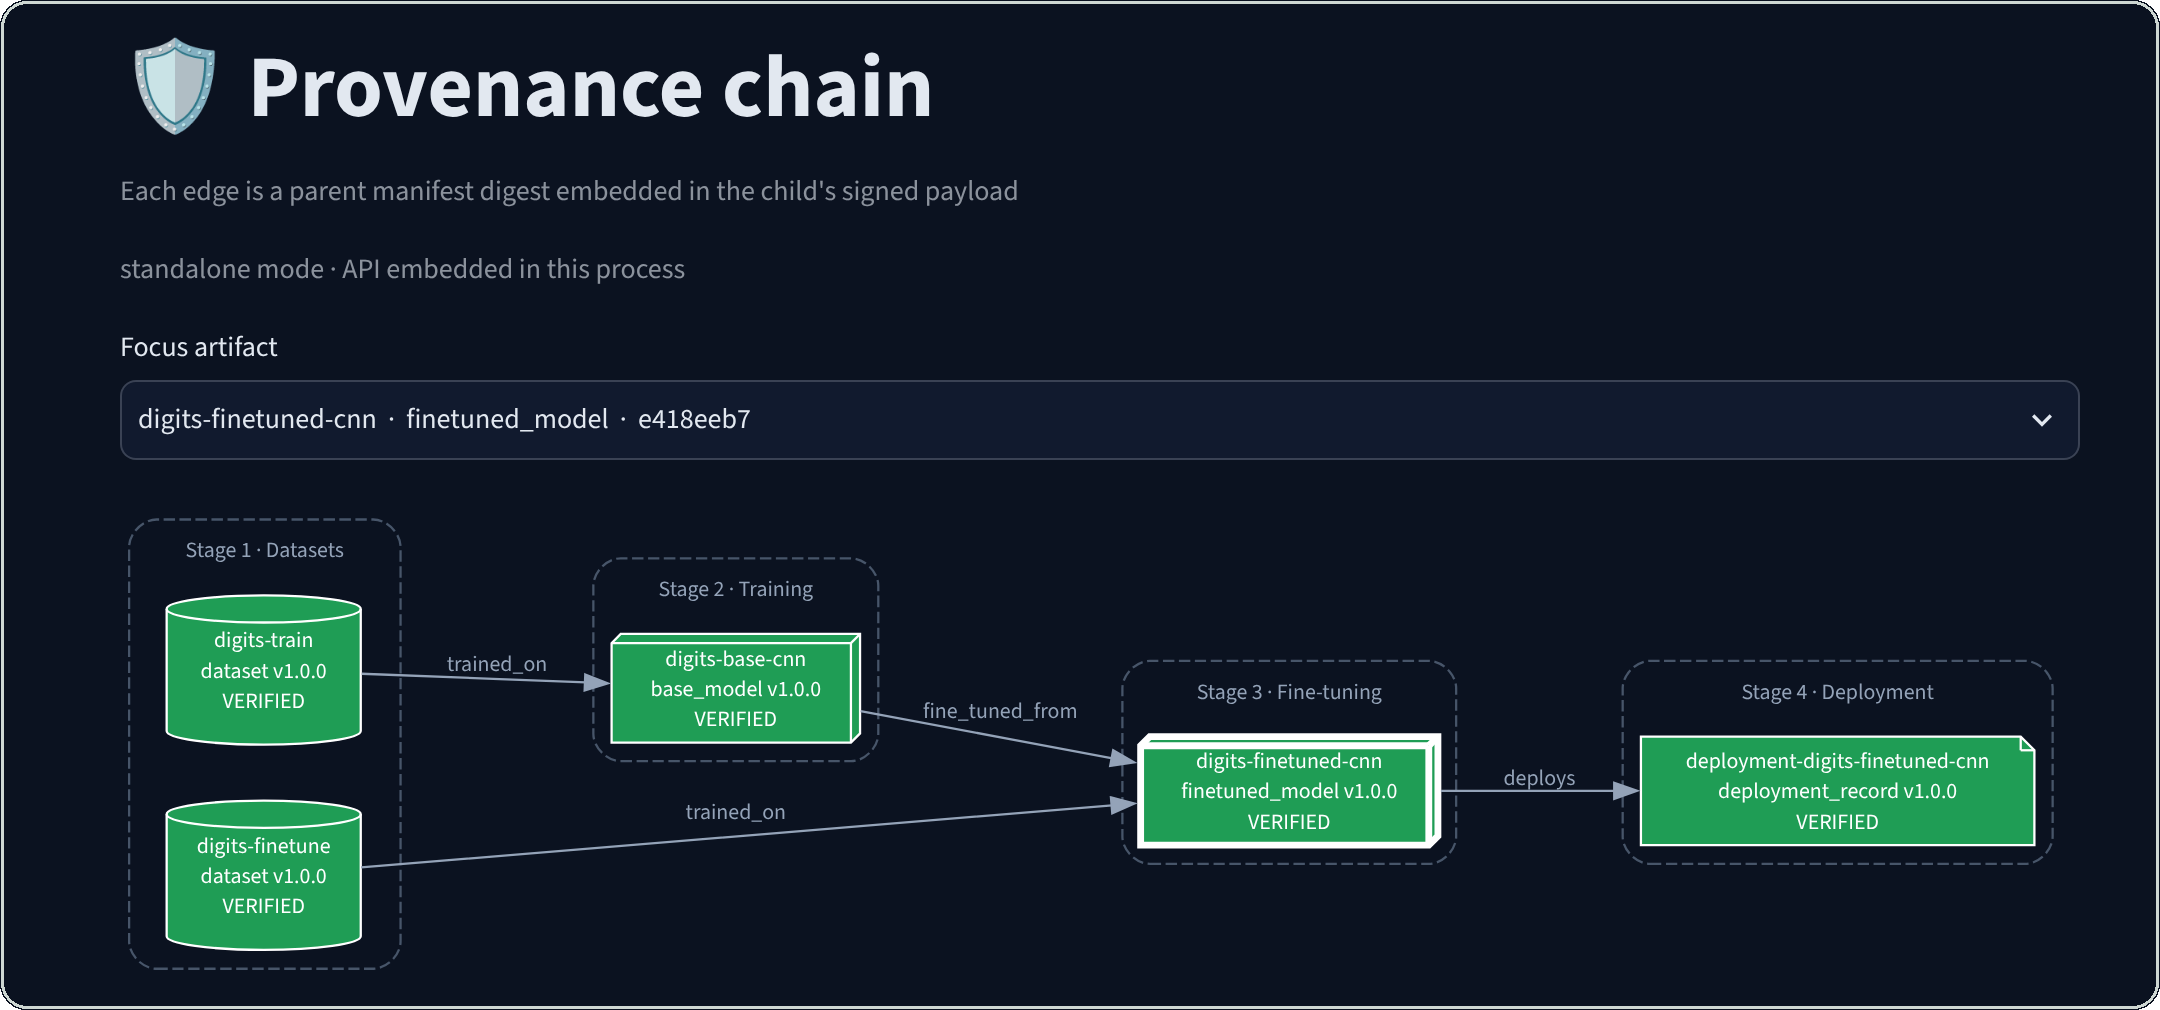
\includegraphics[width=0.86\textwidth]{figures/shot_provenance.png}
\caption{Dashboard, provenance chain page (run of 10~November 2026). Each edge is a parent manifest digest
embedded in the signed payload of the child. The colours show the last verification result stored in the
index; the verifier itself never trusts that stored status.}
\label{fig:dash}
\end{figure}

\subsection{Docker and continuous integration}
A Docker Compose file starts three services on one shared volume: the pipeline, which runs once and exits; the
API on port 8000; and the dashboard on port 8501.

Two GitHub Actions workflows run on every push to the main branch:
\begin{itemize}
\item \code{ci}: the linter, a guard that fails if a private key is committed, and the 168 tests on
  Python~3.11.
\item \code{attest-and-verify}: it creates keys for the run, executes the four-stage attested pipeline and
  fails if the gateway blocks, verifies the deployed model again independently, runs a negative control (one
  flipped byte of the deployed model must give \st{FAILED}), runs the attack scenarios A to D, F and G (43
  variants) and uploads the evidence. An optional job signs with Sigstore; it is disabled by default.
\end{itemize}
This workflow is the automated attestation in CI/CD that the brief suggests: a release is refused unless the
gateway returns \st{VERIFIED}.

\subsection{Test environments}
{\tablefont
\begin{xltabular}{\textwidth}{P{4.9cm}LP{2.3cm}}
\caption{Where the system was executed.}\label{tab:env}\\
\toprule
\headrow\hd{Environment} & \hd{What ran there} & \hd{Date (2026)} \\
\midrule
\endfirsthead
\toprule
\headrow\hd{Environment} & \hd{What ran there} & \hd{Date (2026)} \\
\midrule
\endhead
\bottomrule
\endfoot
Reference environment: cloud Linux container, Intel Xeon at 2.10\,GHz with two logical cores, 8.2\,GB of memory, no GPU, Python 3.13.16, PyTorch 2.15.0 on CPU & The full validation run: linter, 168 tests, pipeline, the 48 variants, every benchmark and figure. Supplementary experiments & 9~November; supplementary runs on 10~November \\
GitHub-hosted runner (Ubuntu, Python 3.11.18, PyTorch 2.15.0) & Both workflows on every push: 168 tests, attested pipeline, negative control, 43 attack variants & 9 and 10~November \\
Team laptop (MacBook Air), Docker & Image build and Compose stack: the four-stage pipeline (\st{VERIFIED}, deployed, clean accuracy 95.0\,\%), the API health check and the dashboard & 16~October \\
Any reader's browser, on the website & Checks V1 and V3 on the deployed model of experiment E2, and the model itself & since 10~November \\
\end{xltabular}}

The benchmarks of Section~\ref{sec:eval} were measured in the reference environment only. Shared CI runners are
not a stable timing environment, and the full test and benchmark run has not been repeated on team hardware.

\subsection{Technologies of the brief}
Python and PyTorch are used throughout. For signing, the brief offers Sigstore, cosign or custom signing with
OpenSSL: we use custom Ed25519 signing on the OpenSSL backend of the \code{cryptography} library, with the
optional Sigstore job in CI. The Merkle tree is our own implementation of RFC~6962. Docker and GitHub Actions
are used as described above. Hyperledger Fabric and blockchain anchoring, both optional, are not used; the
signed trust log takes their place (Section~\ref{sec:trustlog}).

\topsection[sec:eval]{Experimentation and evaluation}

This section covers the experiments of phase~4 and the tests and measurements of phase~5. The scenario scripts
are in \repodir{attacks}, the raw results in \repodir{results} and the dated record of every run in the
experimentation journal (\repofile{docs/09_experimentation_journal.md}).

\subsection{Method}
\textbf{Protocol.} Each attack variant starts from a fresh copy of a clean, fully attested chain. It applies one
manipulation with the access the attacker would have, verifies the targeted artifact with its whole chain, and
records the status, the checks that fired and the wall time of that verification. A variant is correct when the
observed status equals the status predicted before the run. Each experiment has an untouched control, which
must stay \st{VERIFIED}.

\textbf{Backdoor experiments} train real models. The poison is the BadNets trigger \cite{badnets}: a saturated
2 by 2 patch in a corner, stamped on 8\,\% of the training rows (80 rows), whose label is changed to 7. The
\emph{backdoor success rate} is the share of held-out images of the other classes (324 of the 360) that are
classified as 7 once they carry the trigger. The \emph{clean accuracy} is the accuracy on the 360 untouched
held-out images.

\textbf{Environment.} Unless stated otherwise, the numbers come from one run of the whole suite on 9~November
2026 in the reference environment (Table~\ref{tab:env}), with the seed 42. Two supplementary runs were made on
10~November in the same environment; they are identified as such.

\subsection{Every manipulation after signing was detected}
\label{sec:detected}
Figure~\ref{fig:outcomes} shows the 48 variants and Table~\ref{tab:suite} summarises the seven experiments.
All 48 variants ended with the predicted status. Appendix~\ref{app:variants} lists each one.

\begin{figure}[!htb]
\centering
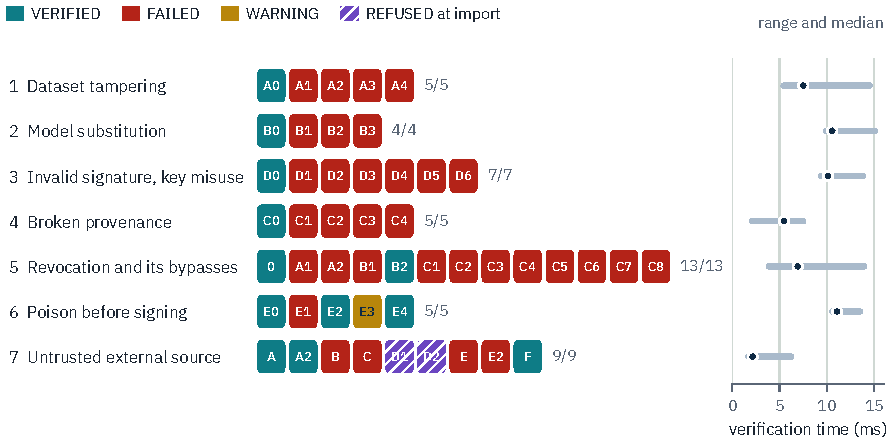
\includegraphics[width=\textwidth]{figures/fig_outcomes.pdf}
\caption{The 48 variants, one tile each, and the verification time of each experiment. The tiles of
experiments 5 and 7 omit the prefixes E5 and E7 of their identifiers. A \st{VERIFIED} tile is either an
untouched control or a case where \st{VERIFIED} was the predicted status, as for E2, E4 and E7-F
(Section~\ref{sec:boundary}).}
\label{fig:outcomes}
\end{figure}

\begin{table}[H]
\caption{The seven experiments: 48 variants, all with the predicted status.}
\label{tab:suite}
\tablefont
\begin{tabularx}{\textwidth}{P{0.55cm}P{4.3cm}rLP{2.35cm}}
\toprule
\headrow\hd{} & \hd{Experiment (scenario)} & \hd{Variants} & \hd{Outcome} & \hd{Checks that fired} \\
\midrule
1 & Dataset tampering (A) & 5 & control \cVER; 4 \cFAIL & V1, V2, V6 \\
2 & Model substitution (B) & 4 & control \cVER; 3 \cFAIL & V1 \\
3 & Invalid signature, key misuse (D) & 7 & control \cVER; 6 \cFAIL & V3, V4, V6 \\
4 & Broken provenance (C) & 5 & control \cVER; 4 \cFAIL & V3, V5, V8 \\
5 & Revocation and its bypasses (F) & 13 & 2 \cVER\ as predicted; 11 \cFAIL, the gateway blocks & V3, V4, V6, V7 \\
6 & Poison before signing (E) & 5 & 3 \cVER\ (E0, E2, E4); 1 \cFAIL\ (E1); 1 \cWARN\ (E3) & V6, V9 \\
7 & Untrusted external source (G) & 9 & 3 \cVER; 4 \cFAIL; 2 \cREF\ at import & V1, V3, V4, V6 \\
\bottomrule
\end{tabularx}
\end{table}

Every manipulation made after signing was rejected, including the subtle ones:
\begin{itemize}
\item \textbf{On datasets:} flipping the labels of five rows, appending one row, or adding a single trailing
  space to one line of a signed file. The report names the changed lines (V1, V2).
\item \textbf{On models:} replacing the file, nudging one weight by $10^{-6}$, which leaves the test accuracy
  unchanged, or saving identical weights again in the pickle format (V1). Integrity is stricter than
  behaviour: a functionally identical model is still rejected.
\item \textbf{On provenance:} deleting a parent record, editing a parent link without signing again, or
  presenting a validly signed model with no dataset ancestry (V5, V3, V8). In variant C2 an insider modifies the
  dataset and signs it again \emph{with the real data-steward key}: the dataset alone verifies, and the model
  that descends from it fails at V5. A legitimate signature cannot rewrite history beneath existing
  descendants.
\item \textbf{On keys:} corrupting or replaying a signature, signing with an unknown or a revoked key, or
  using the data-steward key to sign a model (V3, V4).
\end{itemize}
Revoking an artifact or a key fails every descendant and blocks the deployment, while a dataset signed by
another role still verifies after the training key is revoked: the damage is limited to the revoked key.
Detection, measured as the verification time of the attacked artifact with its chain, took 1.7 to 15.1\,ms,
with a median of 7.5\,ms.

\subsection{Attacks on the trust itself}
Experiment~5 targets the mechanism that decides who is trusted. After a base model is revoked, eight bypasses
(C1 to C8) try to make its fine-tuned descendant verify again:
\begin{itemize}
\item \textbf{Editing the index} (deleting the row of the revoked artifact, C1; deleting the revoked key, C2;
  overwriting the cached status with \st{VERIFIED}, C3). These fail because the verifier never reads a cached
  status and treats a missing row as a revocation it cannot rule out.
\item \textbf{Clearing the \code{revoked} flag in SQLite} (C4). This was the documented limitation of version
  0.3. It now fails: the signed log still says revoked, and the disagreement raises an
  \code{INDEX\_TAMPERING} event (Figure~\ref{fig:bypass}).
\item \textbf{Inserting a rogue key} into the index with the training role and using it to sign a substituted
  model (C5). It fails because the key never entered the signed log.
\item \textbf{Attacking the log}: truncating it to drop the revocation (C6), editing the record in place (C7)
  and deleting the file (C8). All three fail closed: the replay no longer ends at the pinned head, or no longer
  verifies under the root key.
\end{itemize}
What remains trusted is what the threat model declared trusted: whoever holds the root key and can rewrite the
pin controls the trust decisions.

\begin{figure}[!htb]
\centering
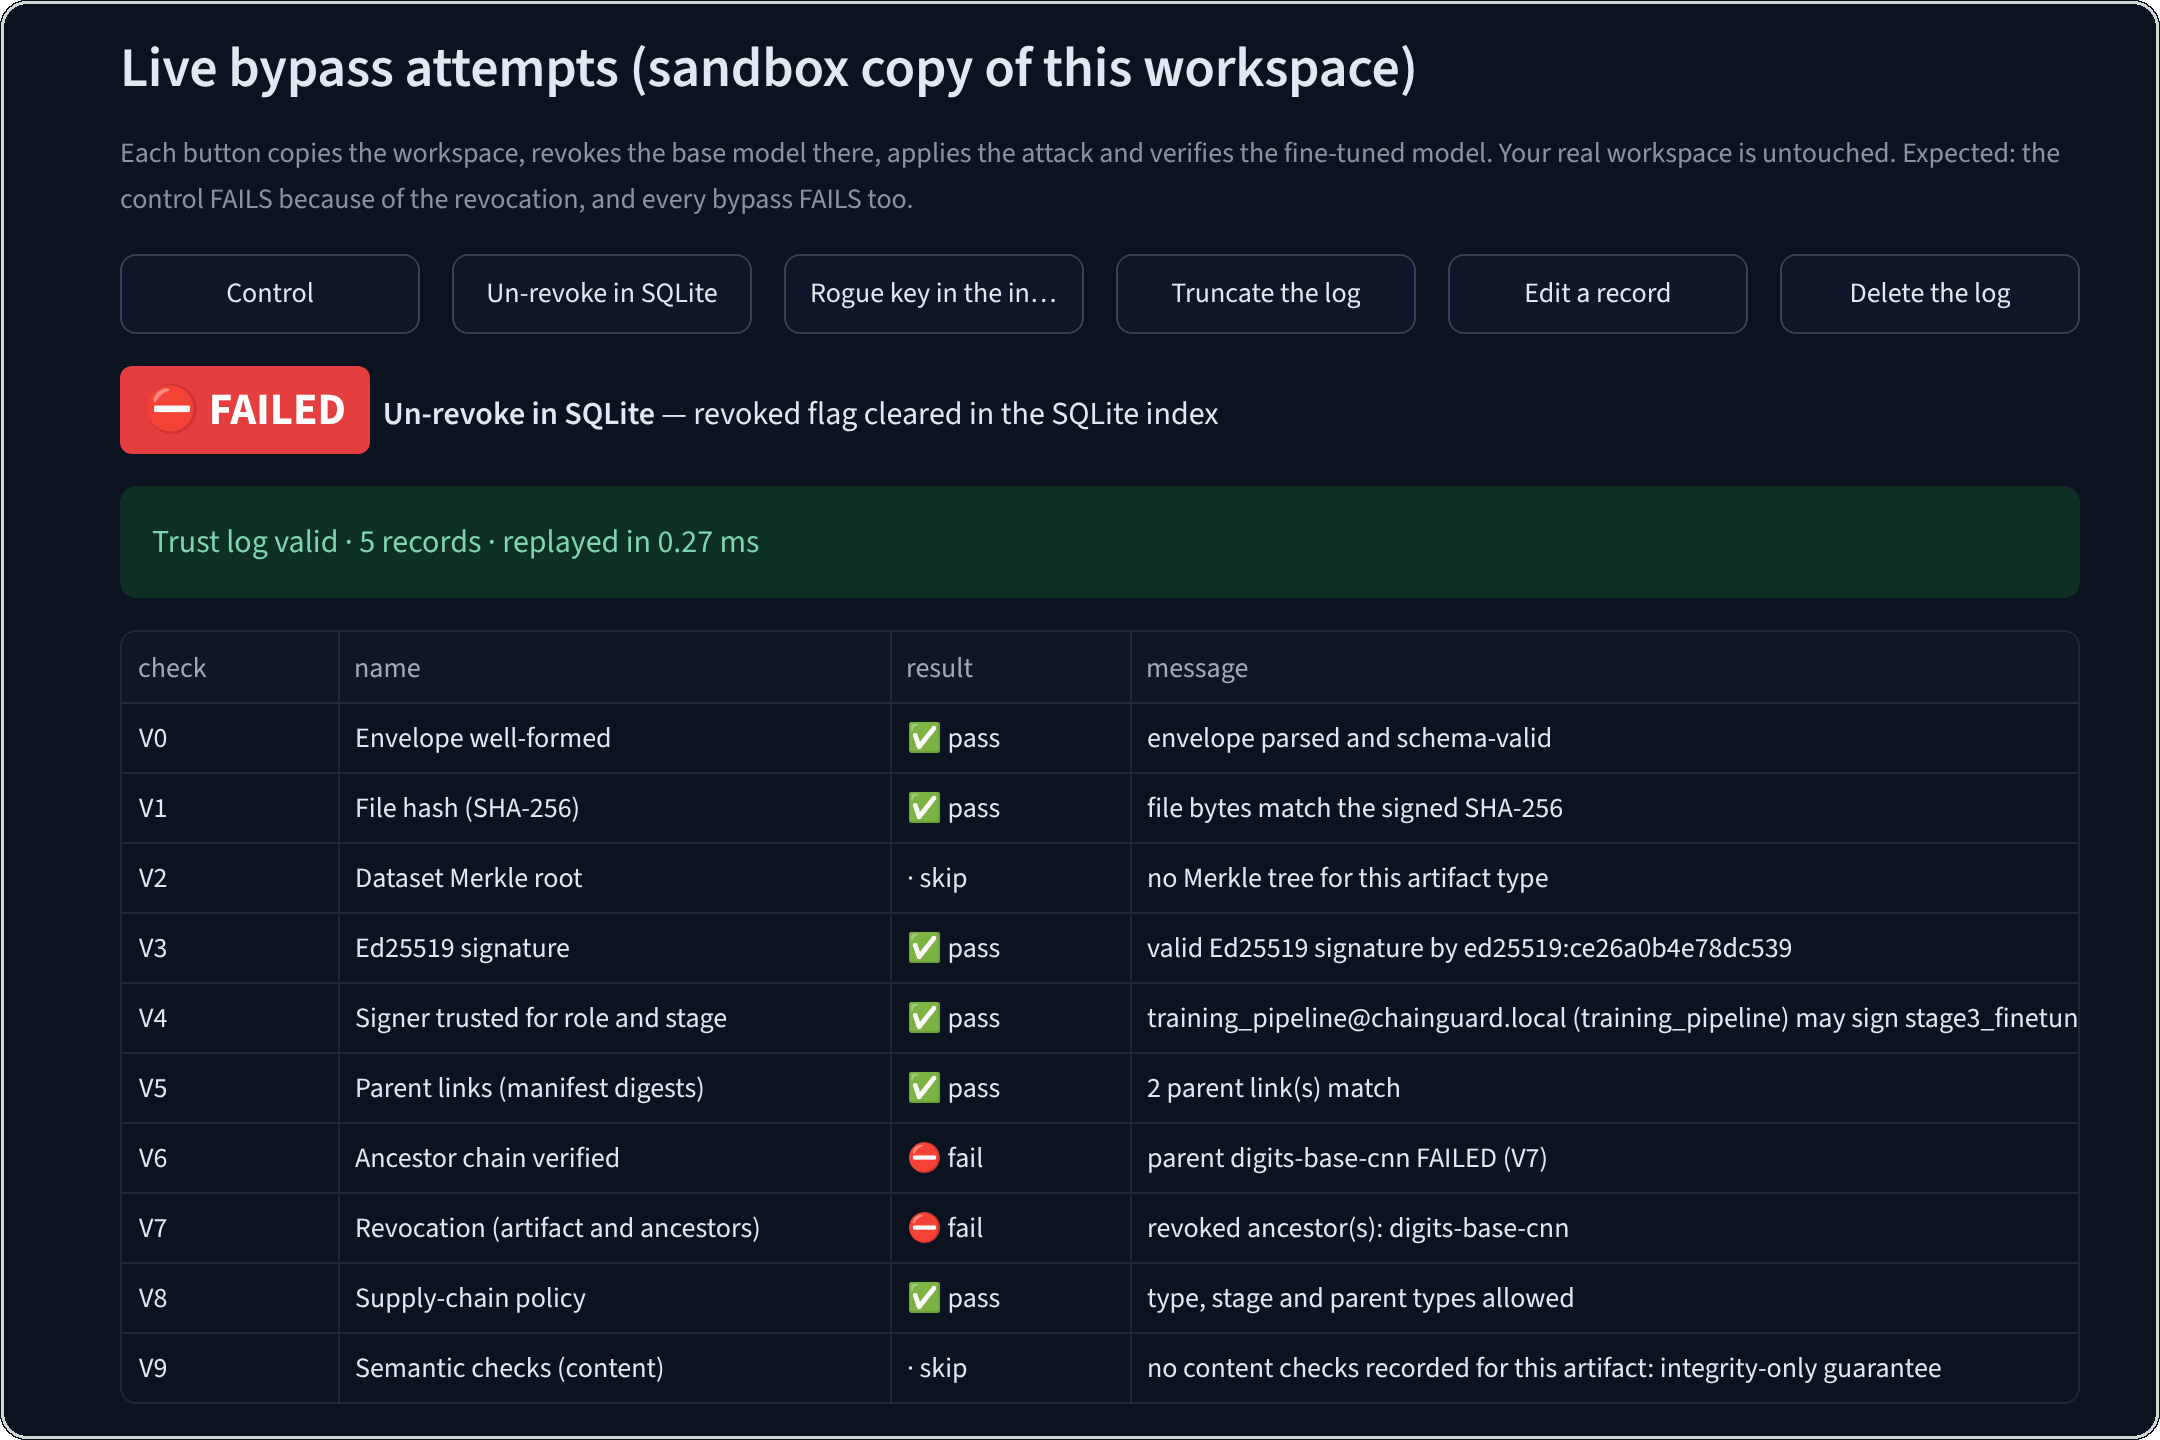
\includegraphics[width=0.72\textwidth]{figures/shot_trustlog.png}
\caption{Dashboard, trust log page: the bypass C4 replayed in a sandbox copy of the workspace (run of
10~November 2026). The revoked flag was cleared in the SQLite index; the fine-tuned model still fails at V6 and
V7 because the signed log is the authority.}
\label{fig:bypass}
\end{figure}

\subsection{Signed is not safe}
\label{sec:boundary}
Experiments 6 and 7 measure what the signature does not cover (Figure~\ref{fig:boundary}).

\begin{figure}[!htb]
\centering
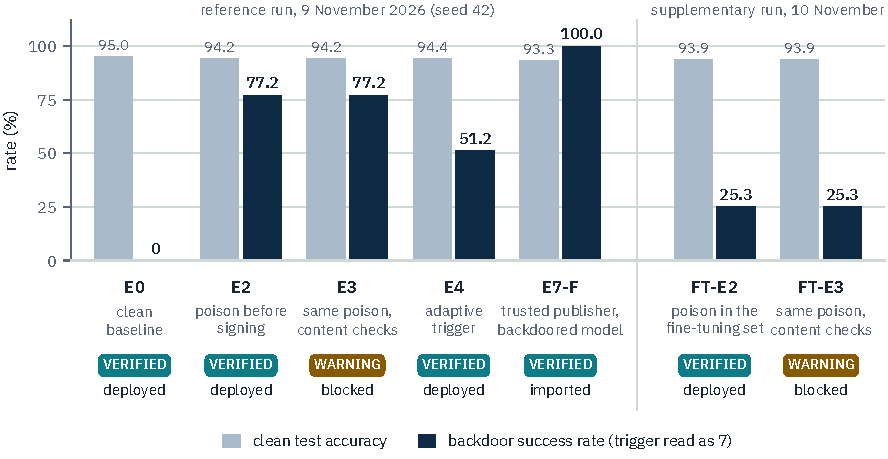
\includegraphics[width=\textwidth]{figures/fig_boundary.pdf}
\caption{Clean accuracy and backdoor success rate of the deployed or imported model, with its verification
status. Signed poison (E2), an adaptive trigger (E4) and the backdoored model of a trusted publisher (E7-F) pass
every cryptographic check. Content checks catch the trigger they know (E3, FT-E3).}
\label{fig:boundary}
\end{figure}

The clean pipeline (E0) deploys a model with a clean accuracy of 95.0\,\% and a backdoor success rate of
0\,\%. Poison injected into the signed dataset \emph{after} signing (E1) fails the chain at V6, as expected.
When the data steward signs a dataset that was poisoned \emph{before} attestation (E2), every check passes. The
fine-tuned model deploys as \st{VERIFIED} with a clean accuracy of 94.2\,\% (339 of the 360 held-out images),
within one point of the clean model, and a backdoor success rate of 77.2\,\% (250 of 324). Ordinary testing
would not reveal it.

With the content checks enabled before signing (E3), the known corner trigger and the shifted label
distribution are flagged. The dataset carries a signed flag, the model verifies with \st{WARNING} and the
gateway blocks it by default: heuristics work as evidence. An adaptive attacker who moves the trigger to a
pattern the checks do not know (E4, a bar on the left edge, 5\,\% of the rows) deploys as \st{VERIFIED} with a
backdoor success rate of 51.2\,\%.

Experiment 7 repeats the lesson at the boundary of the organisation. A backdoored model trained by a
\emph{trusted}, registered publisher (E7-F) imports as \st{VERIFIED} with a clean accuracy of 93.3\,\% and a
backdoor success rate of 100\,\%. The other variants are all rejected: the unknown publisher and the model
modified in transit are \st{FAILED}, the unsigned model and the manifest without its signature are \st{REFUSED}
at import, and the model of a publisher whose key was revoked is \st{FAILED}.

Fine-tuning on clean data weakens the backdoor without removing it: in E2 the base model has a backdoor success
rate of 99.1\,\%, which drops to 77.2\,\% after fine-tuning (99.4\,\% to 51.2\,\% in E4). Fine-tuning is not a
defence to rely on.

\begin{keybox}
\boxtitle{The result in one sentence.} A valid signature proves \emph{who} attested an artifact and \emph{that
nothing changed since}. It transfers trust to the signer and creates none.
\end{keybox}

\subsection{The four example tests of the brief}
The brief gives four example tests. Table~\ref{tab:brieftests} states where each one was run and what was
observed. The first one names the fine-tuning dataset, while experiment 6 poisons the training set of the base
model, so we ran it literally as a supplementary experiment on 10~November (FT-E2 and FT-E3, on the right of
Figure~\ref{fig:boundary}): 8\,\% of the 437 fine-tuning rows (35 rows) receive the corner trigger and the label
7 before the data steward signs them, and the base model is trained on clean data.

{\tablefont
\begin{xltabular}{\textwidth}{P{4.1cm}P{2.6cm}L}
\caption{The four example tests of the brief and what was observed.}\label{tab:brieftests}\\
\toprule
\headrow\hd{Example test of the brief} & \hd{Where} & \hd{Observed} \\
\midrule
\endfirsthead
\toprule
\headrow\hd{Example test of the brief} & \hd{Where} & \hd{Observed} \\
\midrule
\endhead
\bottomrule
\endfoot
Inject a backdoor into a fine-tuning dataset and verify detection failure or success & FT-E2, FT-E3 (and E2 to E4 for the training set) & Detection failure by cryptography: \cVER, deployed, clean accuracy 93.9\,\%, backdoor success 25.3\,\% (base model: 0\,\%). Detection success by the content checks: \cWARN, blocked \\
Substitute a signed model with a tampered version & Experiment 2 (B1 to B3) & Control \cVER. A different model, one weight changed by $10^{-6}$ and the same weights saved as pickle are all \cFAIL\ at V1; the gateway blocks \\
Verify the provenance of a model from an untrusted repository & Experiment 7 (nine variants) & Trusted publisher \cVER. Unknown publisher, model modified after signing and revoked publisher key \cFAIL. Unsigned model and stripped signature \cREF\ at import \\
Measure the attestation overhead on training and inference & Pipeline and inference benchmarks & Attestation 10.7\,ms against 1,288\,ms of training (0.83\,\%). One prediction: 0.084\,ms before and 0.085\,ms after the verified deployment \\
\end{xltabular}}

The backdoor of FT-E2 is weaker than that of E2 (25.3\,\% against 77.2\,\%) because eight epochs of fine-tuning
on 35 poisoned rows teach the model less than fifteen epochs of training on 80. The boundary is the same
wherever the poison enters before signing.

\subsection{Robustness to the random seed}
\label{sec:seeds}
The reference run uses one seed. The seed decides the split of the data, the rows that are poisoned, the
initial weights and the order of the mini-batches, so a single run could be a lucky or an unlucky draw. As a
second supplementary experiment on 10~November, we repeated the four pipeline variants of experiment 6 for ten
other seeds, 0 to 9 (Figure~\ref{fig:seeds}).

\begin{figure}[!htb]
\centering
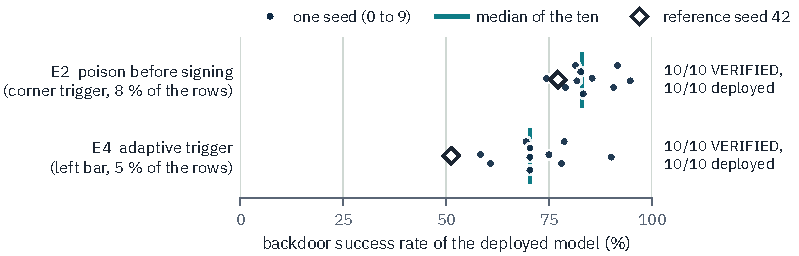
\includegraphics[width=\textwidth]{figures/fig_seeds.pdf}
\caption{Backdoor success rate of the deployed model for ten other seeds. The status never changes. The
reference seed gives the second weakest backdoor of the eleven runs for E2 and the weakest for E4.}
\label{fig:seeds}
\end{figure}

The verification status did not change once in the 40 runs:
\begin{itemize}
\item \textbf{E0, clean:} ten times \st{VERIFIED} and deployed; no content check raised a false alarm; clean
  accuracy 95.8 to 98.6\,\% (median 97.2\,\%); backdoor success rate 0\,\%.
\item \textbf{E2, poison before signing:} ten times \st{VERIFIED} and deployed; backdoor success rate 74.4 to
  94.8\,\% (median 83.0\,\%); clean accuracy 95.8 to 98.3\,\%.
\item \textbf{E3, same poison with content checks:} ten times \st{WARNING} and blocked.
\item \textbf{E4, adaptive trigger:} ten times \st{VERIFIED} and deployed; backdoor success rate 58.3 to
  90.1\,\% (median 70.4\,\%).
\end{itemize}
The run with the seed 42 reproduced the reference results exactly. The figures quoted in this report (77.2\,\%
and 51.2\,\%) are therefore at the low end of what the attack achieves, not a favourable draw.

\subsection{Cost}
\label{sec:cost}
Figure~\ref{fig:cost} gives the cost of each operation and Figure~\ref{fig:scaling} shows how it grows with
the size of what is attested.

\begin{figure}[!htb]
\centering
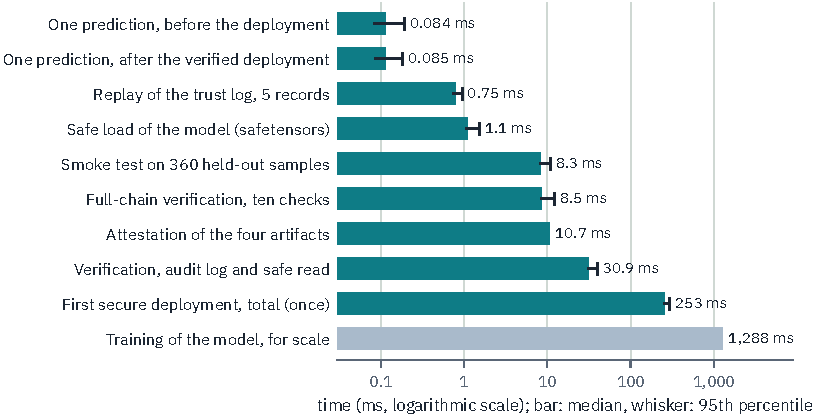
\includegraphics[width=\textwidth]{figures/fig_cost.pdf}
\caption{What attestation costs in the reference environment. Verification happens at deployment, so a
prediction costs the same before and after.}
\label{fig:cost}
\end{figure}

\textbf{Training.} Attesting the four artifacts of the pipeline took 10.7\,ms against 1,288\,ms of training,
or 0.83\,\%. The share depends on the workload and should shrink for larger models, because attestation grows
with the bytes of the artifacts while training grows with the computation.

\textbf{Verification.} A full-chain verification of the fine-tuned model with its three ancestors takes
8.5\,ms (median of 200 runs; 95th percentile 12.2\,ms). Replaying the five-record trust log accounts for
0.16\,ms of it; a first replay, in which every signature is verified, takes 0.75\,ms.

\textbf{Deployment.} The first secure deployment costs 253\,ms, once. The chain verification with its audit
writes and the safe read take 31\,ms, the safetensors load 1.1\,ms and the smoke test 8.3\,ms. The remaining
210\,ms or so go to signing and registering the deployment record, which verifies the chain a second time, and
to event and metric writes.

\textbf{Inference.} A prediction costs 0.084\,ms before and 0.085\,ms after the verified deployment
(medians of 1,000 runs each). Verification is not on the inference path.

\textbf{Storage.} A signed manifest is 1.4 to 3.1\,KB per artifact. The side file that holds the row hashes of
a dataset grows with the number of rows (30 and 68\,KB here).

\begin{figure}[!htb]
\centering
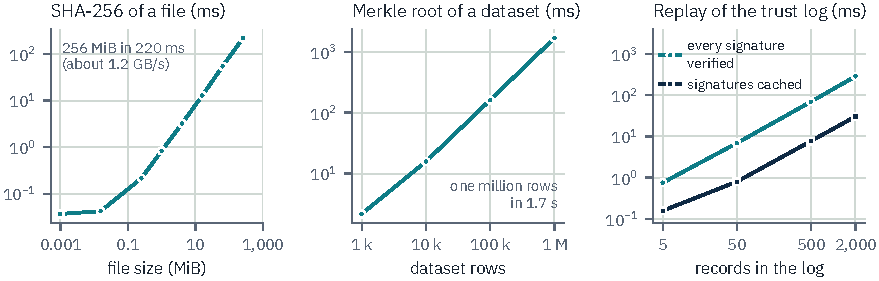
\includegraphics[width=\textwidth]{figures/fig_scaling.pdf}
\caption{How the cost grows. Hashing is linear in the size of the file and dominates for large artifacts;
signing and verifying a signature do not depend on the size (0.04\,ms and 0.12 to 0.14\,ms). Both axes are
logarithmic.}
\label{fig:scaling}
\end{figure}

\textbf{Scaling.} SHA-256 runs at about 1.2\,GB/s, so a model of 256\,MiB hashes in 220\,ms. The Merkle root of
a dataset of one million rows takes 1.7\,s. Replaying the trust log costs about 0.14\,ms per record when every
signature is verified (0.8, 6.9, 69 and 288\,ms for 5, 50, 500 and 2,000 records) and about 15 microseconds
per record with cached signatures. With thousands of records, one would checkpoint a signed snapshot of the
state instead of replaying from the first record.

\subsection{Tests and reproducibility}
\textbf{Automated tests.} 168 tests pass in 36\,s in the reference environment, with none failed and none
skipped: unit tests of hashing, canonical serialisation, signing, manifests, Merkle trees, the policy, the
content checks and the trust log; integration tests of registration and verification, the pipeline, the
revocation experiment, external models, the interoperability export, the API and the scenarios. The suite
grew with the system: 113 tests on 5~October, 143 on 16~October, 168 on 9~November.

\textbf{Continuous integration.} Both workflows passed on the first execution on GitHub (9~November) and on
every push since, on Python 3.11, a different version from the reference environment.

\textbf{Regeneration.} \code{python -m attacks.run\_all} regenerates every table of this section,
\code{python -m scripts.benchmark} and its companions every cost figure, and
\code{report/figures/make\_figures.py} every chart of this report from the result files
(Appendix~\ref{app:repro}).

\textbf{Verification by the reader.} The website serves the signed model of experiment E2, its signed manifest
and the public key. The page checks the file hash (V1) and the Ed25519 signature (V3) in the reader's browser
and runs the network in JavaScript: 339 of 360 clean images correct and 250 of 324 triggered images read as 7,
the figures of E2. Against PyTorch on all 684 inputs, the JavaScript network gave no different prediction.

\subsection{Threats to validity}
\begin{itemize}
\item \textbf{The attack suite is written by the defenders.} It shows that the checks behave as designed
  against the manipulations we thought of, not that no other manipulation exists.
\item \textbf{The model is small.} An 8 by 8 digit classifier shows how large the gap is on a small model, not
  that it has that size for a language model, where poisoning is cheaper \cite{souly2025}.
\item \textbf{The content checks are simple heuristics}, tuned by a defender who knows the trigger. E4 shows
  the cost of that assumption. Stronger detectors would raise the bar and, as adaptive attacks show, not close
  the gap.
\item \textbf{Timings come from one environment.} They were not measured again on team hardware, and shared
  CI runners are not a stable timing environment.
\item \textbf{One trigger family and one dataset.} The seed experiment varies the split, the poisoned rows
  and the initialisation, not the trigger family or the task.
\end{itemize}
None of this touches the central result, which holds by construction: a signature covers bytes, not behaviour.

\topsection[sec:discussion]{Critical analysis}

This section is the critical analysis that phase~5 asks for: what the system guarantees, what it does not, and
how it could be improved.

\subsection{What the system guarantees}
Table~\ref{tab:guarantees} states each guarantee with the mechanism that provides it and the experiment that
tests it.

{\tablefont
\begin{xltabular}{\textwidth}{P{4.7cm}P{4.9cm}L}
\caption{Security guarantees, the mechanism behind each one and the evidence.}\label{tab:guarantees}\\
\toprule
\headrow\hd{Guarantee} & \hd{Mechanism} & \hd{Evidence} \\
\midrule
\endfirsthead
\toprule
\headrow\hd{Guarantee} & \hd{Mechanism} & \hd{Evidence} \\
\midrule
\endhead
\bottomrule
\endfoot
The bytes of an artifact are those that were signed, down to the row for a dataset & SHA-256 of the file and Merkle root of the rows (V1, V2) & Experiments 1 and 2 \\
A known signer, in an authorised role, attested it & Ed25519, trust log, policy (V3, V4, V8) & Experiment 3 \\
The lineage from the dataset to the deployment is intact & Parent digests in the signed payload, recursive verification (V5, V6) & Experiment 4 \\
A withdrawn key or artifact stays withdrawn, even against an insider who can write the database & Signed, hash-chained log with a pinned head (V7) & Experiment 5 \\
What is loaded is what was verified & One read, hashed again, loaded from the same bytes; safetensors only & Variant B3 and the gateway tests \\
An outside model comes from a registered publisher & Publisher key, separate import stage & Experiment 7 \\
\end{xltabular}}

These guarantees hold under the assumption of Section~\ref{sec:threat}: the keys, the pin, the policy and the
verifier are trusted. They hold against every manipulation of our suite, at a cost that an enterprise would not
notice: under one per cent of training time, a few milliseconds per verification and nothing per prediction.

\subsection{What it does not guarantee}
\begin{itemize}
\item \textbf{That signed content is benign.} Poison that is present when the data steward signs is
  faithfully preserved and verified (E2, E4, FT-E2). A backdoored model from a trusted publisher verifies
  (E7-F). The signature moves the question from ``are these the right bytes?'' to ``do I trust this signer?''.
\item \textbf{That a signer is honest or uncompromised.} A stolen key that has not been revoked signs valid
  manifests. A compromised training host can sign a false description of how the weights were produced.
\item \textbf{That a verifier sees the latest revocations.} The trust log is local and has a single writer. A
  verifier that holds an old copy would miss a recent revocation, and the pin file is as critical as the root
  key.
\item \textbf{That content checks find a backdoor.} They flag the trigger family they model and miss the
  others. They are evidence, never proof.
\end{itemize}

\subsection{How the two kinds of evidence fit together}
The design keeps cryptographic evidence and content evidence in separate checks, V0 to V8 on one side and V9 on
the other. A heuristic can never produce \st{FAILED}, and a signature can never produce ``safe''. The status
\st{WARNING} exists for exactly this reason: it says that the integrity is intact and that something about the
content deserves a human decision. Reports also name the external artifacts whose provenance ends at a
publisher. We consider this separation the main lesson of the project for an enterprise. A dashboard that shows
a green \st{VERIFIED} without saying what the status covers invites the wrong conclusion.

\subsection{From this implementation to production}
Several choices fit an eight-week project and would change in production. Table~\ref{tab:production} sets each
one against what a production deployment would use.

{\tablefont
\begin{xltabular}{\textwidth}{P{6.6cm}L}
\caption{Choices that fit an eight-week implementation and what a production deployment would use.}\label{tab:production}\\
\toprule
\headrow\hd{In this implementation} & \hd{In production} \\
\midrule
\endfirsthead
\toprule
\headrow\hd{In this implementation} & \hd{In production} \\
\midrule
\endhead
\bottomrule
\endfoot
Private keys as owner-only files or CI secrets & An HSM or a cloud KMS, or keyless signing with short-lived certificates (Sigstore) \\
Trust log local, with a single writer & Records published to a shared transparency log, or signed snapshots, so that every verifier sees one history \\
Publisher trust is a manual registration of a public key & Identity-based policies (Sigstore, OpenSSF Model Signing) \\
Canonical JSON written in Python (sorted keys, compact) & RFC~8785 \cite{rfc8785}, for signers in other languages \\
API without authentication or TLS & Mutual TLS or OpenID Connect, authorisation per role, keys never on the API host \\
The build environment is a signed claim & Hardware attestation or reproducible training \\
Heuristic content checks (corner trigger, label drift) & Trigger-agnostic detectors and evaluation suites \\
The gateway verifies the chain twice on a first deployment & One verification, reused for the deployment record \\
\end{xltabular}}

\subsection{Improvement paths}
\begin{enumerate}
\item \textbf{Shared history.} Publish the trust-log records and the release root of each deployment to a
  transparency log. This is where a blockchain anchor, optional in the brief, would also fit.
\item \textbf{Keys.} Keyless signing for the roles, hardware-backed root keys, then post-quantum signatures
  through the algorithm field of the manifest.
\item \textbf{Content evidence.} Detectors that do not assume a trigger shape (activation clustering, spectral
  signatures, Neural Cleanse) as further V9 checks, measured against adaptive triggers.
\item \textbf{Scale.} The evaluation repeated on team hardware and with larger models, where hashing dominates
  and the relative overhead should fall.
\item \textbf{Inventory.} The provenance graph exported as a signed bill of materials (CycloneDX or SPDX).
\end{enumerate}

\topsection[sec:valo]{Demonstration, use case and valorisation}

Phase~6 asks for a demonstration or use case and for a conference proposal. This section presents both, with
the website that makes the result checkable by anyone.

\subsection{Demonstration}
The system can be demonstrated in three ways, from the most complete to the most accessible
(Table~\ref{tab:demo}).

{\tablefont
\begin{xltabular}{\textwidth}{P{2.9cm}P{4.4cm}L}
\caption{Three ways to see the system work.}\label{tab:demo}\\
\toprule
\headrow\hd{Demonstration} & \hd{How to start it} & \hd{What it shows} \\
\midrule
\endfirsthead
\toprule
\headrow\hd{Demonstration} & \hd{How to start it} & \hd{What it shows} \\
\midrule
\endhead
\bottomrule
\endfoot
Command-line demonstration, about ten minutes & \code{python -m scripts.demo} & Fifteen steps in a throw-away workspace: a clean chain, the ten checks, \st{VERIFIED}, the provenance tree, a tampered dataset, \st{FAILED}, the gateway blocking, an invalid signature, a revocation, attacks on the index and on the trust log, the poisoned-before-signing limit, a trusted and an untrusted external model, the in-toto export, live metrics \\
Dashboard & \code{make standalone}, then a browser on port 8501 & The same operations by clicking: build the chain, verify, tamper with a real file and restore it, try the bypasses of the trust log in a sandbox, import a model from a trusted, an unknown or an unsigned publisher \\
Website & \href{\site}{\nolinkurl{ai-chainguard.vercel.app}} & The deployed model of experiment E2 verified and run in the browser, a demonstration of the chain with ten attacks, the results, and a 40-second recorded tour of the dashboard \\
\end{xltabular}}

The first two run the complete system on the presenter's machine. The website is a static page: it runs no
server of ours. The two checks it performs and the model itself execute in the visitor's browser, on the real
files of the run (Figure~\ref{fig:web}). The page is available in English, French, Spanish, German and Hindi.

\begin{figure}[!htb]
\centering
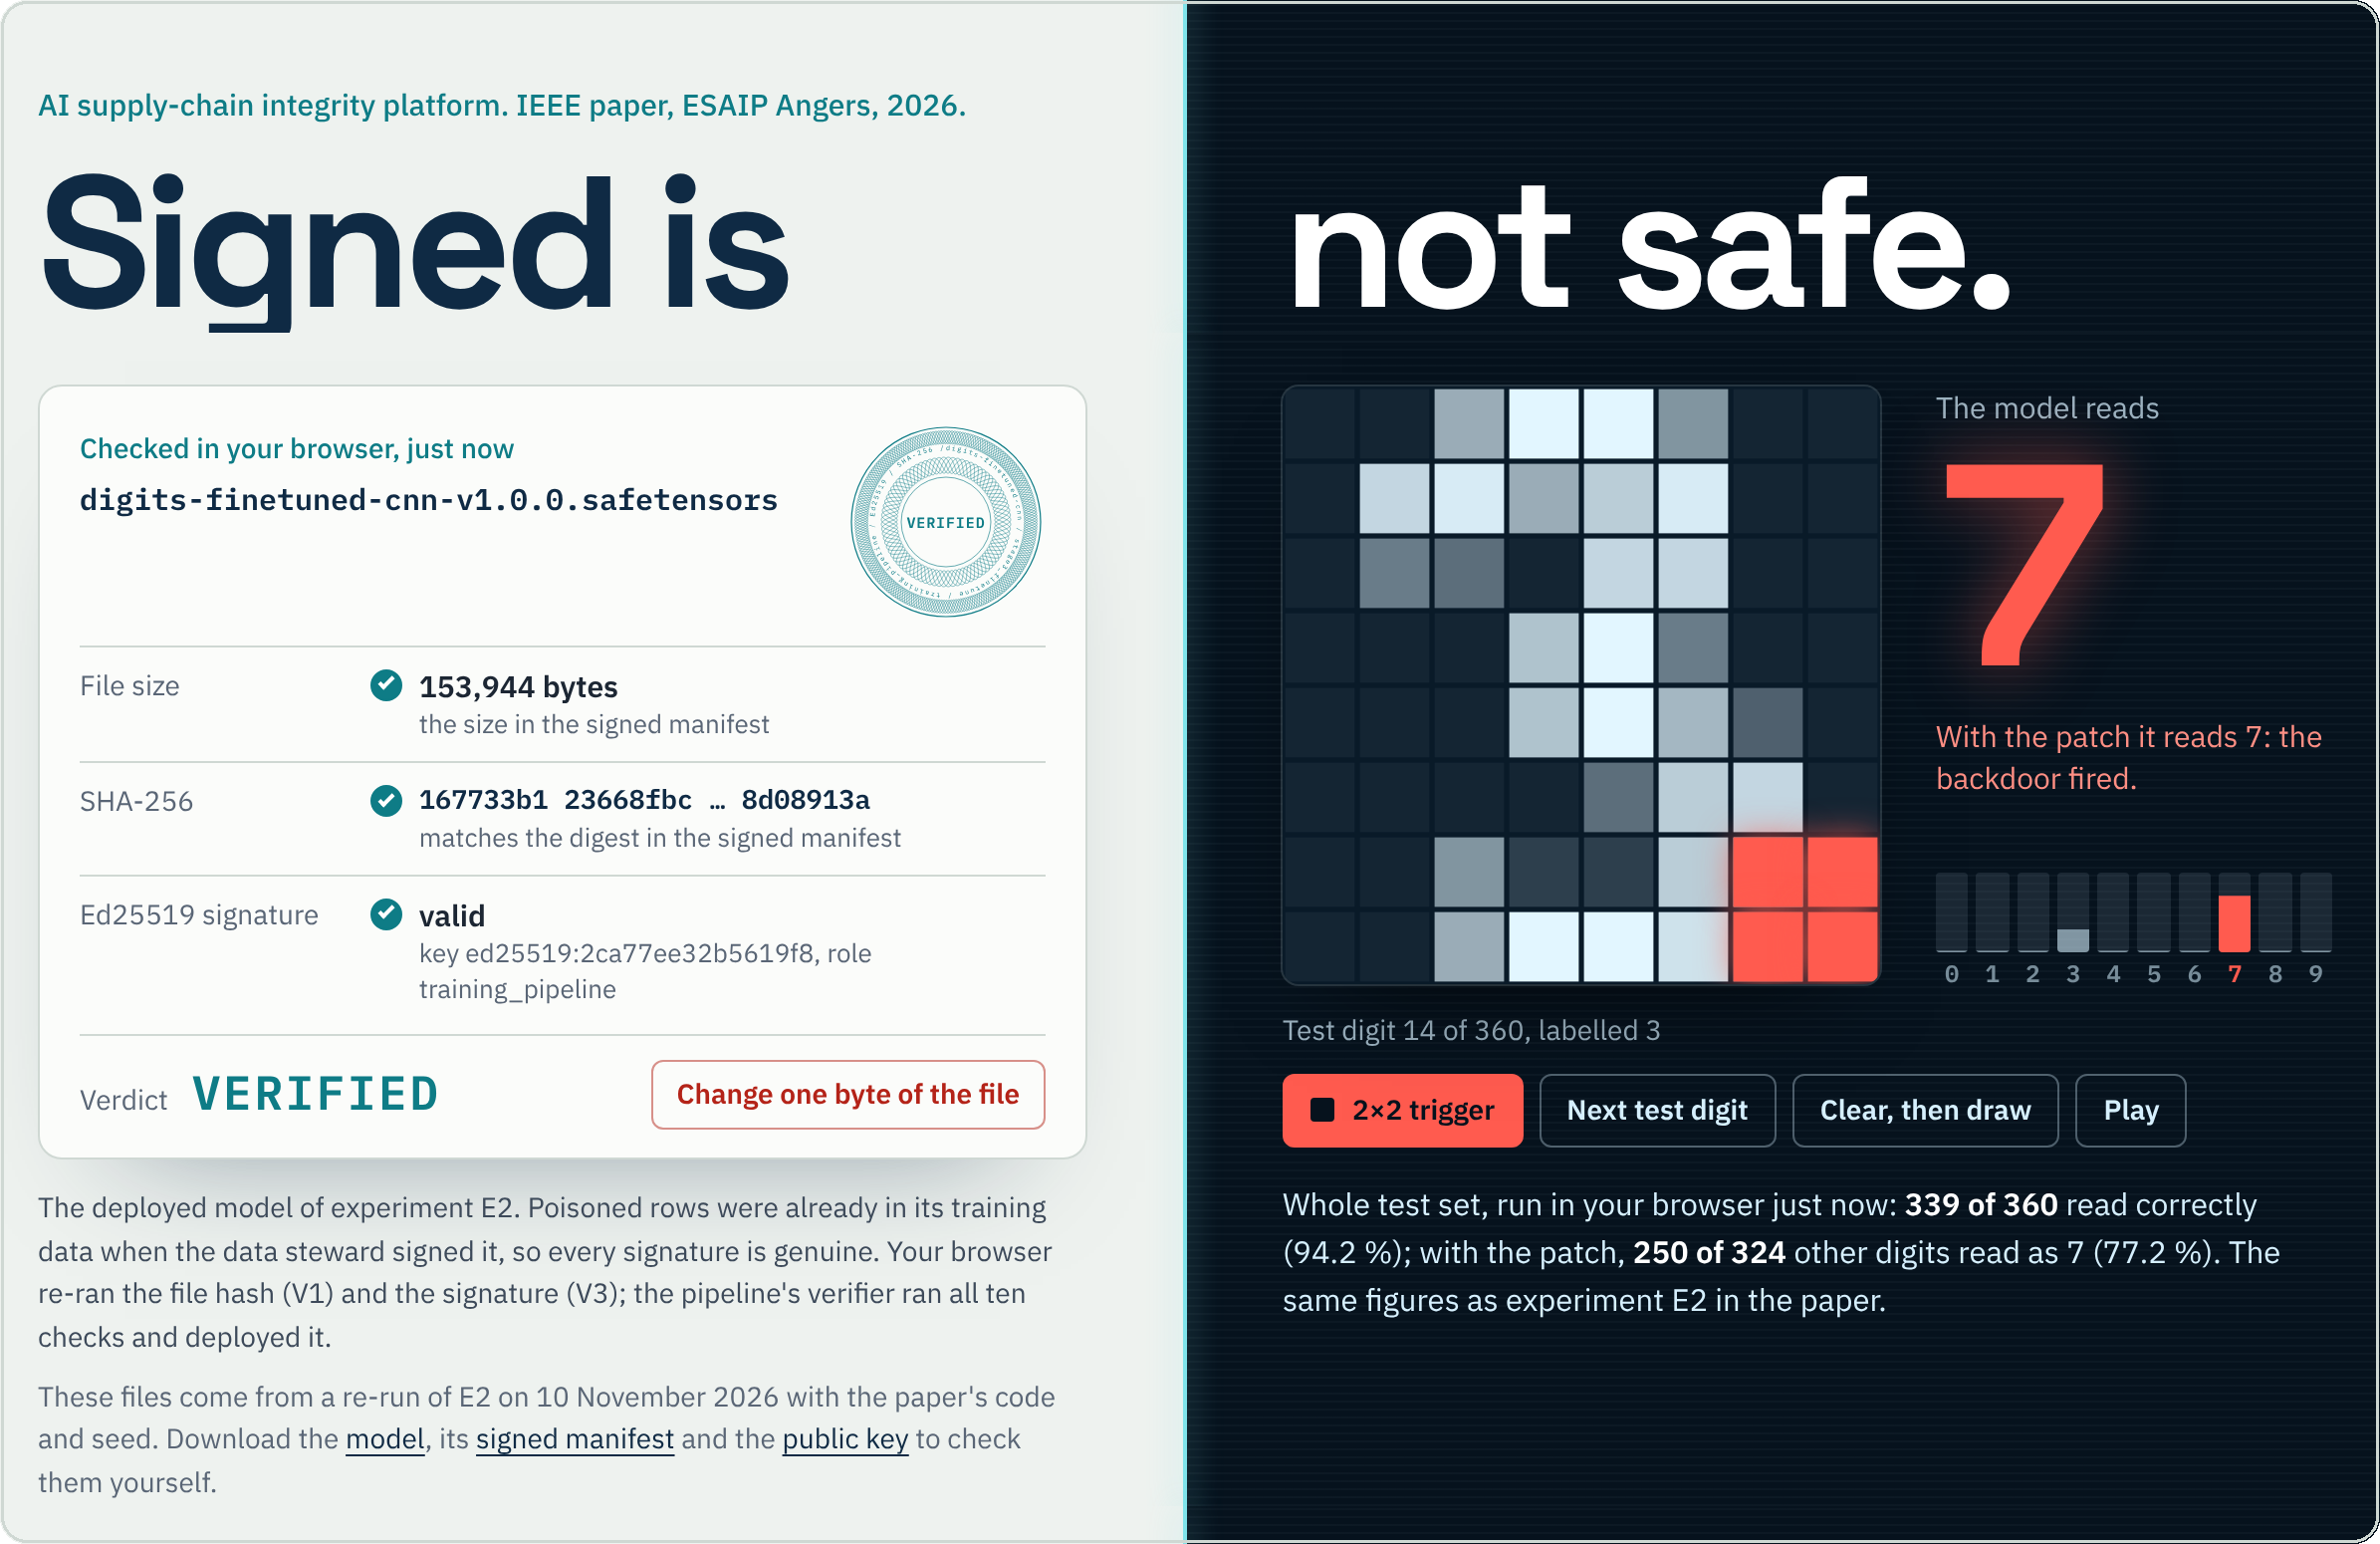
\includegraphics[width=0.8\textwidth]{figures/shot_website.png}
\caption{The website (10~November 2026). Left: the deployed model of experiment E2 passes the hash and
signature checks in the browser. Right: the same model reads a 3 as a 7 once the trigger is stamped on it.}
\label{fig:web}
\end{figure}

\subsection{Use case: a model taken from a hub and fine-tuned in the enterprise}
A team wants to fine-tune a pretrained model from an outside publisher on internal data and deploy it.
\begin{enumerate}
\item The security team registers the public key of the publisher. The model is imported: an unsigned file
  is refused, an altered one fails verification and is quarantined, and the accepted model is labelled as
  external.
\item The data steward registers the internal dataset. Content checks run, and their result is signed with
  the data.
\item The training pipeline fine-tunes and signs the result, whose manifest embeds the digests of the dataset
  and of the external model.
\item At deployment the gateway verifies the whole chain, loads the verified bytes and signs a deployment
  record with a release root.
\item Months later the publisher announces that its key was compromised. The release manager revokes the key
  in the trust log. From that moment every model that descends from that publisher fails verification, and the
  gateway refuses to deploy them again, even if an insider edits the database.
\item During the investigation, the release root of each deployment tells the auditors exactly which dataset,
  which base model and which keys were behind the model in production, and the attestations can be handed to
  tools that read in-toto or SLSA.
\end{enumerate}
Steps 1 to 5 are exercised by experiments 5 and 7. Step 6 uses the deployment record and the export of
Section~\ref{sec:design}. The use case also shows the limit: if the publisher's model was already backdoored
when it was signed, steps 1 to 4 succeed (variant E7-F).

\subsection{Conference proposal}
The common framework of the projects asks for a conference proposal with a title, an abstract and a targeted
venue (\repofile{docs/13_conference_proposal.md}). We went one step further and wrote the full paper, six pages
in IEEE conference format (\repodir{paper}).

\textbf{Title.} \emph{Signed Is Not Safe: Measuring the Boundary Between Cryptographic Integrity and Semantic
Trust in AI Supply Chains.}

\textbf{Abstract, in short.} The paper presents the attestation chain, then measures the boundary of its
guarantees with the 48 variants: every manipulation after signing is detected, while a dataset poisoned before
signing verifies and deploys. It argues that AI supply-chain controls must report cryptographic evidence and
content evidence separately.

\textbf{Venues.} Table~\ref{tab:venues} lists the venues we target.

\begin{table}[H]
\caption{Targeted venues. Deadlines and page limits must be checked on each call for papers before submitting.}
\label{tab:venues}
\tablefont
\begin{tabularx}{\textwidth}{P{5.1cm}LP{2.4cm}}
\toprule
\headrow\hd{Venue} & \hd{Why it fits} & \hd{Format} \\
\midrule
ACM SCORED, workshop on software supply-chain security, co-located with ACM CCS (first choice) & The contribution is a supply-chain mechanism and a measurement of its boundary: attestation, in-toto, SLSA, Sigstore & Workshop paper \\
ACM AISec, workshop on artificial intelligence and security, co-located with ACM CCS & Security of machine-learning systems, poisoning and backdoors & Workshop paper \\
IEEE SaTML, conference on secure and trustworthy machine learning & Trustworthy machine learning, measurement of defences & Conference paper \\
C\&ESAR (Rennes) or RESSI & The French security research and teaching community; a French version of the paper exists & Conference or short paper \\
\bottomrule
\end{tabularx}
\end{table}

\subsection{Value for an enterprise security team}
Three properties make the work usable beyond the course. It needs no outside service: it runs offline, with
files and one SQLite database. It speaks the formats that software supply-chain tools already consume (in-toto
statements, DSSE envelopes, SLSA provenance). And it states its limit in the product itself: a status that
means ``exactly what trusted signers attested'', a separate status for content doubts, and a label on models
whose provenance ends outside the organisation.

\topsection[sec:project]{Project management}

\subsection{Plan and milestones}
The scoping note planned four milestones over the eight weeks, with an end-to-end chain first so that
integration would never be left to the end. Table~\ref{tab:plan} compares the plan with the dated evidence.

{\tablefont
\begin{xltabular}{\textwidth}{P{4.4cm}P{1.9cm}L}
\caption{Milestones planned in the scoping note and when each one was reached.}\label{tab:plan}\\
\toprule
\headrow\hd{Milestone} & \hd{Planned} & \hd{Reached} \\
\midrule
\endfirsthead
\toprule
\headrow\hd{Milestone} & \hd{Planned} & \hd{Reached} \\
\midrule
\endhead
\bottomrule
\endfoot
Minimum chain: register, hash, sign, verify, detect tampering & Week 2 & 5~October: version 0.2 already attested the four stages, with 113 tests and 26 attack and control variants in five scenarios. First progress report \\
Four-stage chain with roles, policy and revocation & Week 4 & 16~October: version 0.3 added the revocation experiment and external models, with 143 tests and 44 variants. The Compose stack ran on a team laptop. Second progress report \\
Attack scenarios and measurements & Weeks 5 to 7 & 26 variants on 5~October, 44 on 16~October, 48 in the final run of 9~November, each time with the cost measurements \\
Report, paper and demonstration & Week 8 & 9 and 10~November: version 0.4 with the signed trust log and the export, full validation run, public repository with both CI workflows passing, the paper, the website and this report \\
\end{xltabular}}

Each full run is kept: the results of 5~October and 16~October are archived unchanged in the repository
(\repodir{results}), and the experimentation journal has one dated entry per run, which is never deleted.

\subsection{Team and ownership}
Table~\ref{tab:team} gives the area each member is responsible for. It describes ownership, not a record of
individual contributions.

\begin{table}[H]
\caption{Team roles and areas of ownership.}
\label{tab:team}
\tablefont
\begin{tabularx}{\textwidth}{P{3.1cm}P{3.5cm}L}
\toprule
\headrow\hd{Member} & \hd{Role} & \hd{Owns} \\
\midrule
Karan DESHMUKH & Technical lead, security architecture & Architecture and integration, verifier and trust-log design, external-model design, deployment gateway, API, interoperability export, coordination, paper \\
JOGI Sudheer reddy & AI and ML engineer & Dataset and training pipeline, backdoor experiments (experiments 6 and 7), inference benchmark \\
DAMA Dola Krishna & Testing, documentation and quality & Test suite, experimentation journal, collection of results, validation script, dashboard support, reports \\
MEKALA Rambabu & Security and DevOps engineer & Hashing, signatures, key and publisher-key handling, revocation and trust-log operations, Docker, CI/CD \\
\bottomrule
\end{tabularx}
\end{table}

\subsection{Reporting to the referent}
The brief asks for a detailed weekly progress report. Karan DESHMUKH sent it to the referent by email. Two
formal progress reports mark the main steps: the report on the initial period (5~October 2026) and Progress
Report~2 (16~October 2026). The progress update for version 0.4 (9~November 2026) is in the repository
(\repofile{docs/16_progress_update_v0.4.md}). The two formal reports are archived with this report so that the
progression can be checked.

\subsection{Method}
\textbf{Evidence rule.} From the first report, a feature is reported as completed only when code and
repeatable execution evidence exist, and every number is tied to the run that produced it. This report follows
the same rule.

\textbf{Use of AI assistance.} As stated in each progress report, the code was produced with AI-assisted code
generation and validated by execution: tests, complete validation runs in the reference environment, the CI
workflows and the Docker run on a team laptop. The design decisions, the experiments, their analysis and the
conclusions are the responsibility of the team.

\subsection{Difficulties and lessons}
\begin{itemize}
\item \textbf{Our own experiment broke our design.} In version 0.3 the revocation experiment showed that
  clearing one flag in the database undid a revocation. We reported it as a limitation on 16~October and
  removed it in version 0.4 with the signed trust log. Lesson: attack your own trust anchors, and write the
  limitation down before fixing it.
\item \textbf{A detector must be measured on clean data first.} The first version of the corner-trigger check
  flagged 11 clean digits. Requiring the minimum of the four pixels instead of their mean brought the false
  alarms to zero, on the reference split and on the ten other seeds of Section~\ref{sec:seeds}.
\item \textbf{Run the automation before trusting it.} The CI guard against committed private keys matched
  its own search pattern in the workflow file and would have failed on every run. Executing the workflow steps
  locally found the bug before the first run on GitHub.
\item \textbf{One environment is not enough.} Docker could not run in the reference environment, so the
  Compose stack was executed on a team laptop. Timings still come from one environment.
\item \textbf{Saying what a result does not mean is part of the result.} Keeping \st{VERIFIED} from being read
  as ``safe'' shaped the statuses, the dashboard and the wording of every report.
\end{itemize}

\topsection[sec:conclusion]{Conclusion and future work}

We built an attestation chain for AI pipelines. It links datasets, base models, external models, fine-tuned
models and deployments through signed manifests that embed the digests of their parents. It enforces who may
sign which stage, keeps trust and revocation in a signed, pinned, append-only log, and gates deployment on a
verification of the whole chain. The system is complete from the command line to the dashboard, tested by 168
automated tests and by two CI workflows, and documented phase by phase as the brief requires.

On 48 attack and control variants, every manipulation made after signing was detected, including the bypasses
aimed at the index and at the log itself. The cost is under one per cent of training time, 8.5\,ms per
verification and nothing per prediction. The answer to the first sub-question of the project is therefore yes:
an enterprise can verify cryptographically that an artifact, and everything it descends from, is exactly what
authorised parties attested.

The same suite answers the second sub-question. Poison that is present before signing verifies and deploys,
with a backdoor success rate of 77.2\,\% in the reference run and of 74 to 95\,\% for ten other seeds. Content
checks catch the trigger they know and miss an adaptive one. A backdoored model from a trusted publisher
verifies. Cryptographic attestation is necessary for an AI supply chain and it is not sufficient: it must be
combined with evidence about content, and the two must be reported separately.

\textbf{Future work.} In order of priority: publish the trust log and the release roots to a shared
transparency log; replace long-lived keys by keyless signing and hardware-backed roots; repeat the evaluation
on team hardware and with larger models; add trigger-agnostic detectors as further content checks and measure
them against adaptive triggers; export the provenance graph as a signed bill of materials. The paper is ready
to be adapted to the page limit of the first targeted venue.

% Generated by report/tools/order_refs.py from references_src.tex. Do not edit by hand.
\FloatBarrier\needspace{12\baselineskip}
\addsec{References}\label{sec:refs}\vspace{-0.45\baselineskip}%
{\color{cgrule}\rule{\textwidth}{0.6pt}}\par\vspace{0.15\baselineskip}
{\sffamily\fontsize{8.5}{11.3}\selectfont\setlength{\itemsep}{2.2pt}\raggedright
\makeatletter\renewcommand*{\bib@heading}{}\makeatother
\begin{thebibliography}{99}
\setlength{\itemsep}{2.2pt}\setlength{\parskip}{0pt}
\bibitem{pytorch2022} PyTorch team, ``Compromised PyTorch-nightly dependency chain between December 25th and December 30th, 2022,'' Dec. 31, 2022. [Online]. Available: \url{https://pytorch.org/blog/compromised-nightly-dependency/}. Accessed: Nov. 9, 2026.
\bibitem{jfrog2024} D. Cohen, JFrog Security Research, ``Data scientists targeted by malicious Hugging Face ML models with silent backdoor,'' Feb. 2024. [Online]. Available: \url{https://jfrog.com/blog/data-scientists-targeted-by-malicious-hugging-face-ml-models-with-silent-backdoor/}. Accessed: Nov. 9, 2026.
\bibitem{carlini2024} N. Carlini et al., ``Poisoning web-scale training datasets is practical,'' in \emph{Proc. IEEE Symp. Security and Privacy (SP)}, 2024, pp. 407-425.
\bibitem{souly2025} A. Souly et al., ``Poisoning attacks on LLMs require a near-constant number of poison samples,'' arXiv:2510.07192 [cs.LG], Oct. 2025.
\bibitem{aiact2024} European Parliament and Council, ``Regulation (EU) 2024/1689 of 13 June 2024 laying down harmonised rules on artificial intelligence (Artificial Intelligence Act),'' \emph{Off. J. Eur. Union}, L, 2024/1689, Jul. 12, 2024, Art. 15(5).
\bibitem{slsa11} OpenSSF, ``SLSA specification v1.1: Supply-chain Levels for Software Artifacts,'' Apr. 2025. [Online]. Available: \url{https://slsa.dev/spec/v1.1/}. Accessed: Nov. 9, 2026.
\bibitem{intoto2019} S. Torres-Arias, H. Afzali, T. K. Kuppusamy, R. Curtmola, and J. Cappos, ``in-toto: Providing farm-to-table guarantees for bits and bytes,'' in \emph{Proc. 28th USENIX Security Symp.}, 2019, pp. 1393-1410.
\bibitem{sigstore2022} Z. Newman, J. S. Meyers, and S. Torres-Arias, ``Sigstore: Software signing for everybody,'' in \emph{Proc. ACM SIGSAC Conf. Computer and Communications Security (CCS)}, 2022, pp. 2353-2367.
\bibitem{oms2025} OpenSSF, ``Model Signing v1.0,'' Apr. 2025. [Online]. Available: \url{https://github.com/sigstore/model-transparency}. Accessed: Nov. 9, 2026.
\bibitem{badnets} T. Gu, B. Dolan-Gavitt, and S. Garg, ``BadNets: Identifying vulnerabilities in the machine learning model supply chain,'' arXiv:1708.06733 [cs.CR], 2017.
\bibitem{rl2025} K. Zanki, ReversingLabs, ``Malicious ML models discovered on Hugging Face platform,'' Feb. 2025. [Online]. Available: \url{https://www.reversinglabs.com/blog/rl-identifies-malware-ml-model-hosted-on-hugging-face}. Accessed: Nov. 9, 2026.
\bibitem{nistairmf} NIST, ``Artificial Intelligence Risk Management Framework (AI RMF 1.0),'' NIST AI 100-1, Jan. 2023.
\bibitem{atlas} MITRE, ``ATLAS technique AML.T0010: AI supply chain compromise.'' [Online]. Available: \url{https://atlas.mitre.org/techniques/AML.T0010}. Accessed: Nov. 9, 2026.
\bibitem{owaspml} OWASP Foundation, ``OWASP Machine Learning Security Top Ten, ML06:2023 ML supply chain attacks.'' [Online]. Available: \url{https://owasp.org/www-project-machine-learning-security-top-10/docs/ML06_2023-AI_Supply_Chain_Attacks.html}. Accessed: Nov. 10, 2026.
\bibitem{rfc8032} S. Josefsson and I. Liusvaara, ``Edwards-Curve Digital Signature Algorithm (EdDSA),'' RFC 8032, IETF, Jan. 2017.
\bibitem{dsse} Secure Systems Lab, ``DSSE: Dead Simple Signing Envelope, protocol v1.'' [Online]. Available: \url{https://github.com/secure-systems-lab/dsse}. Accessed: Nov. 9, 2026.
\bibitem{intotoattest} in-toto project, ``in-toto Attestation Framework: Statement v1.'' [Online]. Available: \url{https://github.com/in-toto/attestation}. Accessed: Nov. 9, 2026.
\bibitem{tuf2010} J. Samuel, N. Mathewson, J. Cappos, and R. Dingledine, ``Survivable key compromise in software update systems,'' in \emph{Proc. ACM Conf. Computer and Communications Security (CCS)}, 2010, pp. 61-72.
\bibitem{rfc6962} B. Laurie, A. Langley, and E. Kasper, ``Certificate Transparency,'' RFC 6962, IETF, Jun. 2013.
\bibitem{modelcards} M. Mitchell et al., ``Model cards for model reporting,'' in \emph{Proc. Conf. Fairness, Accountability, and Transparency (FAT*)}, 2019, pp. 220-229.
\bibitem{datasheets} T. Gebru et al., ``Datasheets for datasets,'' \emph{Commun. ACM}, vol. 64, no. 12, pp. 86-92, 2021.
\bibitem{cyclonedx15} OWASP CycloneDX, ``Introducing OWASP CycloneDX v1.5: Advanced bill of materials standard empowering transparency, security, and compliance,'' Jun. 2023. [Online]. Available: \url{https://cyclonedx.org/news/cyclonedx-v1.5-released}. Accessed: Nov. 10, 2026.
\bibitem{spdx3} The Linux Foundation, ``SPDX 3.0 revolutionizes software management in systems with enhanced functionality and streamlined use cases,'' Apr. 2024. [Online]. Available: \url{https://www.linuxfoundation.org/press/spdx-3-revolutionizes-software-management-in-systems-with-enhanced-functionality-and-streamlined-use-cases}. Accessed: Nov. 10, 2026.
\bibitem{activation} B. Chen et al., ``Detecting backdoor attacks on deep neural networks by activation clustering,'' in \emph{Proc. AAAI Workshop on Artificial Intelligence Safety (SafeAI)}, 2019.
\bibitem{spectral} B. Tran, J. Li, and A. Madry, ``Spectral signatures in backdoor attacks,'' in \emph{Advances in Neural Information Processing Systems (NeurIPS)}, vol. 31, 2018.
\bibitem{neuralcleanse} B. Wang et al., ``Neural Cleanse: Identifying and mitigating backdoor attacks in neural networks,'' in \emph{Proc. IEEE Symp. Security and Privacy (SP)}, 2019, pp. 707-723.
\bibitem{strip} Y. Gao, C. Xu, D. Wang, S. Chen, D. C. Ranasinghe, and S. Nepal, ``STRIP: A defence against trojan attacks on deep neural networks,'' in \emph{Proc. Annu. Computer Security Applications Conf. (ACSAC)}, 2019, pp. 113-125.
\bibitem{safetensors} Hugging Face, ``Safetensors: a simple, safe way to store and distribute tensors,'' documentation; security audit by Trail of Bits, 2023. [Online]. Available: \url{https://huggingface.co/docs/safetensors}. Accessed: Nov. 9, 2026.
\bibitem{rfc8785} A. Rundgren, B. Jordan, and S. Erdtman, ``JSON Canonicalization Scheme (JCS),'' RFC 8785, IETF, Jun. 2020.
\end{thebibliography}}

\clearpage
\appendix
\renewcommand*{\sectionformat}{\textcolor{cgteal}{Appendix \thesection}\hspace{0.7em}}
\addtocontents{toc}{\protect\vspace{6pt}}
\addtocontents{toc}{\protect\noindent{\protect\sffamily\protect\small\protect\color{cgmuted}Appendices, outside the page count of the report}\protect\par}

\section{Requirements of the brief and where each one is met}
\label{app:trace}
\vspace{-0.45\baselineskip}{\color{cgrule}\rule{\textwidth}{0.6pt}}\par\vspace{0.15\baselineskip}
The table follows the brief of Projet Applicatif 2 line by line. The same checklist, with direct links to the
files, is \repofile{docs/18_requirements_checklist.md}.

{\tablefont
\begin{xltabular}{\textwidth}{P{4.95cm}P{1.35cm}LP{1.3cm}}
\toprule
\headrow\hd{Requirement of the brief} & \hd{Section} & \hd{Evidence in the repository} & \hd{Status} \\
\midrule
\endfirsthead
\toprule
\headrow\hd{Requirement of the brief} & \hd{Section} & \hd{Evidence in the repository} & \hd{Status} \\
\midrule
\endhead
\bottomrule
\endfoot
\multicolumn{4}{l}{\textbf{\color{cgnavy}Common framework}} \\*
Project over two months, eight weeks & \ref{sec:project} & Week 1 from 21 September 2026; final day 10 November 2026 & Done \\
Detailed weekly progress report to the referent & \ref{sec:project} & Sent by email; progress reports of 5 and 16 October; \code{docs/14}, \code{docs/16} & Done \\
Demonstration of the realisation & \ref{sec:valo} & \code{scripts/demo.py} (15 steps), dashboard, website; \code{docs/15}, \code{docs/17} & Ready \\
Conference proposal: title, abstract, targeted venue & \ref{sec:valo} & \code{docs/13}; full paper in \code{paper/} & Done \\
\midrule
\multicolumn{4}{l}{\textbf{\color{cgnavy}Pedagogical objectives}} \\*
Understand the threats specific to AI supply chains & \ref{sec:scoping}, \ref{sec:soa} & \code{docs/02} section 2, \code{docs/04} & Done \\
Analyse the risks for model provenance, dataset lineage and pipeline integrity & \ref{sec:threat} & \code{docs/04}: assets, actors, trust boundaries, STRIDE, residual risks & Done \\
Study cryptographic signing, hash chains and Merkle trees & \ref{sec:soa}, \ref{sec:design} & \code{docs/02} sections 3 and 4, \code{docs/07} & Done \\
Design a coherent attestation architecture & \ref{sec:design} & \code{docs/05}, \code{docs/06}, \code{docs/07} & Done \\
Implement a functional system & \ref{sec:impl} & Source code, 168 tests, two CI workflows passing & Done \\
Evaluate the results objectively & \ref{sec:eval}, \ref{sec:discussion} & \code{results/}, \code{docs/08}, including the measured limit & Done \\
\midrule
\multicolumn{4}{l}{\textbf{\color{cgnavy}Phase 1: scoping and problem definition}} \\*
Scope for the attestation of AI artifacts in an enterprise; a clear cybersecurity problem & \ref{sec:intro}, \ref{sec:scoping} & \code{docs/01} sections 1, 2 and 6 & Done \\
Assets: datasets, pretrained models, fine-tuned weights, training scripts, inference APIs & \ref{sec:scoping} & \code{docs/01} section 3, \code{docs/04} section 1 & Done \\
Threats: data poisoning, backdoor injection, model substitution, pipeline compromise & \ref{sec:scoping}, \ref{sec:threat} & \code{docs/01} section 4, \code{docs/04} & Done \\
Deliverable: scoping note of 2 to 3 pages & \ref{sec:scoping} & \code{docs/01\_scoping\_note.md} & Done \\
\midrule
\multicolumn{4}{l}{\textbf{\color{cgnavy}Phase 2: state of the art and critical analysis}} \\*
Attacks: direct poisoning, backdoored base models, environment poisoning & \ref{sec:soa} & \code{docs/02} sections 2.1 to 2.3 & Done \\
Existing solutions: cryptographic signing, SLSA for ML, model cards, Sigstore & \ref{sec:soa} & \code{docs/02} sections 3 to 5 & Done \\
Compare open-source, industrial and academic approaches; identify the limitations & \ref{sec:soa} & \code{docs/02} sections 8 and 9, \code{docs/03} & Done \\
Deliverables: synthesis of 3 to 5 pages, comparative table, argued justification of the approach & \ref{sec:soa} & \code{docs/02} (justification in section 10), \code{docs/03} & Done \\
\midrule
\multicolumn{4}{l}{\textbf{\color{cgnavy}Phase 3: solution design}} \\*
Provenance and integrity architecture for AI artifacts & \ref{sec:design} & \code{docs/05} & Done \\
Signing, verification and revocation mechanisms & \ref{sec:design} & \code{docs/07}; \code{chainguard/trustlog.py} & Done \\
Justified technical choices & \ref{sec:soa}, \ref{sec:design} & \code{docs/05} section 7, \code{docs/02} section 10 & Done \\
Deliverables: architecture diagrams, functional and technical description, attack scenarios & \ref{sec:design} & \code{docs/05} (six diagrams), \code{docs/06}, \code{docs/07}, \code{docs/08} & Done \\
Indicative architecture: hash chain or Merkle tree & \ref{sec:design} & Hash-linked manifests and row-level Merkle roots for datasets & Done \\
Indicative architecture: signing of models and datasets at each pipeline stage & \ref{sec:design} & Ed25519 manifests for datasets, base model, fine-tuned model and deployment record & Done \\
Indicative architecture: blockchain anchoring (optional) & \ref{sec:soa} & Not built; a signed, hash-chained, pinned trust log instead, justified in \code{docs/02} sections 4 and 10 & Optional, not built \\
Indicative architecture: CI/CD integration for automated attestation & \ref{sec:impl} & \code{.github/workflows/attest-and-verify.yml} & Done \\
Indicative architecture: verification API for deployment gateways & \ref{sec:impl} & \code{api/} and \code{deployment/gateway.py} & Done \\
\midrule
\multicolumn{4}{l}{\textbf{\color{cgnavy}Phase 4: implementation and experimentation}} \\*
Simulated ML pipeline & \ref{sec:impl} & \code{ml\_pipeline/} & Done \\
Attestation across at least three pipeline stages & \ref{sec:design} & Four stages & Done \\
Documented code and scripts & \ref{sec:impl} & \code{README.md}, docstrings, \code{scripts/}, \code{docs/07} & Done \\
Description of the test environment & \ref{sec:impl} & \code{docs/09}, \code{results/validation\_logs/environment.txt} & Done \\
Experimentation journal & \ref{sec:eval} & \code{docs/09\_experimentation\_journal.md} & Done \\
Technologies: Python, PyTorch; Sigstore, cosign or custom signing with OpenSSL; Merkle tree library; Docker, GitHub Actions; Hyperledger Fabric (optional) & \ref{sec:impl} & Python and PyTorch; custom Ed25519 signing on OpenSSL and an optional Sigstore job; own RFC 6962 implementation; \code{docker/}; \code{.github/workflows/}; Hyperledger not used & Done \\
\midrule
\multicolumn{4}{l}{\textbf{\color{cgnavy}Phase 5: testing, evaluation and critical analysis}} \\*
Test against realistic attack scenarios & \ref{sec:eval} & 48 variants in seven experiments, \code{attacks/}, \code{docs/08} & Done \\
Measure detection rates and overhead & \ref{sec:eval} & \code{results/attacks/}, \code{results/metrics/} & Done \\
Deliverables: test results as logs, tables and graphs & \ref{sec:eval} & \code{results/validation\_logs/}, \code{results/attacks/summary.csv}, \code{results/figures/}, \code{report/figures/} & Done \\
Critical analysis of the guarantees and the limitations; improvement paths & \ref{sec:discussion} & Paper sections V and VI, \code{docs/04} (residual risks) & Done \\
The four example tests & \ref{sec:eval} & Table~\ref{tab:brieftests} of this report & Done \\
\midrule
\multicolumn{4}{l}{\textbf{\color{cgnavy}Phase 6: reporting and valorisation}} \\*
Final report of about 30 pages & all & This document; source in \code{report/} & Done \\
Oral defence & \ref{sec:valo} & Presentation guide (\code{docs/17}) and slides prepared & Ready \\
Demonstration or use case & \ref{sec:valo} & Demonstration script, dashboard, website & Done \\
Conference proposal & \ref{sec:valo} & \code{docs/13}, \code{paper/} & Done \\
\midrule
\multicolumn{4}{l}{\textbf{\color{cgnavy}Expected results}} \\*
A functional attestation system; a complete engineering approach with threat modelling; a critical analysis of the results; work that can be valorised in an enterprise security context & all & The repository, documents \code{01} to \code{09}, this report, the paper and the website & Done \\
\end{xltabular}}

\needspace{14\baselineskip}
\section{The 48 variants}
\label{app:variants}
\vspace{-0.45\baselineskip}{\color{cgrule}\rule{\textwidth}{0.6pt}}\par\vspace{0.15\baselineskip}
Reference run of 9~November 2026. For every variant the observed status equals the status predicted before the
run. The time is that of the verification of the attacked artifact with its chain.

\makeatletter{\tablefont
\begin{xltabular}{\textwidth}{P{1.3cm}LP{1.75cm}P{2.45cm}r}
\toprule
\headrow\hd{Variant} & \hd{Manipulation} & \hd{Status} & \hd{Checks that fired} & \hd{Time (ms)} \\
\endfirsthead
\toprule
\headrow\hd{Variant} & \hd{Manipulation} & \hd{Status} & \hd{Checks that fired} & \hd{Time (ms)} \\
\endhead
\bottomrule
\endfoot
\@@input sections/gen_variants.tex 
\end{xltabular}}\makeatother

\needspace{20\baselineskip}
\section{A signed manifest}
\label{app:manifest}
\vspace{-0.45\baselineskip}{\color{cgrule}\rule{\textwidth}{0.6pt}}\par\vspace{0.15\baselineskip}
The manifest of the fine-tuned model of the reference run, as stored on disk. Three provenance fields are
shortened here for space (marked by three dots), so this printed version is not the signed payload itself. The
two parents are the base model and the fine-tuning dataset, each named by its manifest digest.

\begin{lstlisting}
{
  "payload_type": "application/vnd.chainguard.manifest+json; version=1",
  "payload": {
    "schema_version": "1.0",
    "artifact_id": "9f25b977-0aa0-4aa8-a149-4f19d79f3ee2",
    "artifact_name": "digits-finetuned-cnn",
    "artifact_type": "finetuned_model",
    "version": "1.0.0",
    "pipeline_stage": "stage3_finetune",
    "subject": {
      "uri": "artifacts/models/digits-finetuned-cnn-v1.0.0.safetensors",
      "sha256": "1f1448ea86c028d9d36e80b764eca9a52368fdf9847cb901db394f338b16a0ae",
      "size_bytes": 153944,
      "media_type": "application/safetensors",
      "merkle": null
    },
    "parents": [
      { "artifact_id": "a85de012-e158-4221-85e7-826ff7749d5f",
        "manifest_digest": "sha256:1f930c8538ccf7ed0ef95813eed5d8fad5741bad7956e8fab1faf6d8ea82fd21",
        "relation": "fine_tuned_from" },
      { "artifact_id": "3c4e300b-12fe-4883-89c6-cdb3ce96758a",
        "manifest_digest": "sha256:6959cdaa0188c84cf87e0b9b28dfa6d84c0e1f38b68193f5fb49133f212048ea",
        "relation": "trained_on" }
    ],
    "provenance": {
      "source": "internal fine-tuning pipeline",
      "builder": "ml_pipeline/finetune.py",
      "parameters": { "epochs": 8, "lr": 0.0005, "batch_size": 64, "seed": 42 },
      "metrics": { ... },
      "input_verification": { ... },
      "environment": { "python": "3.13.16", "chainguard": "0.4.0", "torch": "2.15.0+cu132", ... }
    },
    "semantic_checks": [],
    "created_at": "2026-11-09T09:26:46Z",
    "signer": {
      "identity": "training_pipeline@chainguard.local",
      "role": "training_pipeline",
      "key_id": "ed25519:cec6a3e317c4a128"
    }
  },
  "signatures": [
    { "key_id": "ed25519:cec6a3e317c4a128", "algorithm": "Ed25519",
      "sig": "n5sYF5FF/diG4Vp88bYcJcsciUHMH9cHh+N8uvt+vXnMwpxp/DCfUaGCEpX3G0yhkzudUNgZMkF3Fuban7syBA=="
    }
  ],
  "manifest_digest": "sha256:133c0274c7b49c52fb8a58504bb8f090a7a28853d8f1e0be98ffd73004f1e0e9"
}
\end{lstlisting}

The last field is a convenience copy. The verifier never trusts it: it recomputes the digest from the payload.

\section{Reproducing the results}
\label{app:repro}
\vspace{-0.45\baselineskip}{\color{cgrule}\rule{\textwidth}{0.6pt}}\par\vspace{0.15\baselineskip}
From a clone of the repository, with Python 3.11 or later:

\begin{lstlisting}
make install          # dependencies, PyTorch for CPU
make keys             # one Ed25519 key pair per role
make pipeline         # the four-stage attested pipeline and the deployment gateway
make attacks          # the 48 variants of the seven experiments
make benchmark        # cost of hashing, signing and verification
make test             # the 168 tests
python -m scripts.e2_finetune_poison      # supplementary run: poison in the fine-tuning set
python -m scripts.seed_robustness         # supplementary run: ten other seeds
python report/figures/make_figures.py     # the charts of this report
make demo             # the ten-minute demonstration
make standalone       # the dashboard, on port 8501
docker compose -f docker/docker-compose.yml up --build    # pipeline, API and dashboard in containers
make validate LABEL="<machine>"           # the whole validation sequence, with its logs
\end{lstlisting}

\section{Deliverables and where to find them}
\label{app:deliverables}
\vspace{-0.45\baselineskip}{\color{cgrule}\rule{\textwidth}{0.6pt}}\par\vspace{0.15\baselineskip}
{\tablefont
\begin{tabularx}{\textwidth}{P{4.0cm}L}
\toprule
\headrow\hd{Deliverable} & \hd{Location} \\
\midrule
This report, PDF and LaTeX source & \repodir{report} \\
Website & \url{\site} \\
Source code, tests, Docker and CI files & \url{\repo} \\
Conference paper, PDF and LaTeX source & \repodir{paper} \\
Conference proposal & \repofile{docs/13_conference_proposal.md} \\
Scoping note, state of the art, comparative table, threat model, architecture, functional and technical descriptions, attack scenarios, experimentation journal & \repodir{docs}, documents \code{01} to \code{09} \\
Requirements checklist & \repofile{docs/18_requirements_checklist.md} \\
Results: logs, tables, figures, archived earlier runs & \repodir{results} \\
Demonstration runbook & \repofile{docs/15_professor_demo_10min.md} \\
Earlier progress reports of 5 and 16 October 2026 & Folder \emph{Previous reports} of the hand-in package \\
\bottomrule
\end{tabularx}}

\end{document}
